\documentclass[
  	%draft,    % omit title page, listings, and particular chapters selected below using include only
	%german,   % titles for a thesis in German, A4 paper
	print,    % the printed version does not use colored links
	%final,    % removes all TODOs
]{tex/ttthesis}
\geometry{a4paper}

% Color Scheme http://colorschemedesigner.com/#3w40I--ALK-K-
% Base Color of the OVGU INF logo, tetraed, -45
\definecolor{blue1}{RGB}{0,105,180} % gray 95
\definecolor{blue2}{RGB}{40,87,121}
\definecolor{blue3}{RGB}{0,57,97}
\definecolor{blue4}{RGB}{76,166,230}
\definecolor{blue5}{RGB}{136,191,230}
\definecolor{orange1}{RGB}{255,144,0} % gray 133
\definecolor{orange2}{RGB}{171,121,56}
\definecolor{orange3}{RGB}{137,78,0}
\definecolor{orange4}{RGB}{255,181,84}
\definecolor{orange5}{RGB}{255,210,151}
\definecolor{green1}{RGB}{11,215,0} % gray 75
\definecolor{green2}{RGB}{52,144,48}
\definecolor{green3}{RGB}{6,116,0}
\definecolor{green4}{RGB}{88,241,80}
\definecolor{green5}{RGB}{148,241,143}
\definecolor{red1}{RGB}{253,0,6} % gray 86
\definecolor{red2}{RGB}{170,56,59}
\definecolor{red3}{RGB}{136,0,3}
\definecolor{red4}{RGB}{254,84,88}
\definecolor{red5}{RGB}{254,151,154}

\definecolor{background}{named}{white}
\definecolor{bgborder}{named}{black}
\definecolor{comment}{named}{red3}

\definecolor{blue}{named}{blue1}
\definecolor{green}{named}{green1}
\definecolor{red}{named}{red1}
\definecolor{orange}{named}{orange1}
 
\definecolor{pdflinkcolor}{named}{blue3}
\definecolor{pdfcitecolor}{named}{green3}

\usepackage{listings} % source code listings

%\renewcommand\lstlistingname{Quelltext}

\lstdefinestyle{java}{
%code formatting
	language=Java,
	tabsize=4,
	breaklines=false,
	basicstyle=\fontfamily{pcr}\footnotesize\selectfont,
	commentstyle=\fontshape{it}\color{darkgray}\selectfont,
	keywordstyle=\fontseries{b}\selectfont,
	stringstyle=\fontfamily{cmr}\selectfont,
%line numbering
	numbers=left,
	numberstyle=\footnotesize,
%frame properties
	captionpos=b,
	frame=single,%trblTRBL
	framesep=3pt,
	xleftmargin=4pt,
	xrightmargin=4pt,
	rulecolor=\color{bgborder},
}

\usepackage{pgfplots}
\usepackage{tikz}
	\usetikzlibrary{arrows,positioning,backgrounds,fit,trees} 
	\usetikzlibrary{fadings,shapes.geometric}
	\usetikzlibrary{decorations,scopes,calc,decorations.pathreplacing}

% Tortendiagramme
\newcommand{\slice}[4]{
  \pgfmathparse{0.5*#1+0.5*#2}
  \let\midangle\pgfmathresult

  % slice
  \draw[thick,
	%fill=background
	] (0,0) -- (#1:1) arc (#1:#2:1) -- cycle;

  % outer label
  \node[label=\midangle:#4] at (\midangle:1) {};

  % inner label
  \pgfmathparse{min((#2-#1-10)/110*(-0.3),0)}
  \let\temp\pgfmathresult
  \pgfmathparse{max(\temp,-0.5) + 0.8}
  \let\innerpos\pgfmathresult
  \node at (\midangle:\innerpos) {#3};
}
\newcommand{\mypiechart}[2]{
	\begin{tikzpicture}[scale=#1]
		\newcounter{a}
		\newcounter{b}
		\foreach \p/\t in {#2}
			{
				\setcounter{a}{\value{b}}
				\addtocounter{b}{\p}
				\slice{\thea/100*360}
							{\theb/100*360}
							{\p\%}{\t}
			}
	\end{tikzpicture}
}

% surrounding TODOs with this command, gives you the ability to remove all if necessary
\iffinal{
	\newcommand{\todo}[1]{}
	\newcommand{\todots}{}
}{
	\newcommand{\todo}[1]{{\color{comment}\textit{[#1]}}}
	\newcommand{\todots}{\todo{\ldots}}
}

% propositional formulas
\newcommand{\pand}{\wedge}
\newcommand{\por}{\vee}
\newcommand{\pnot}{\neg}
\newcommand{\pequals}{\Leftrightarrow}
\newcommand{\pimplies}{\Rightarrow}
\newcommand{\pnimplies}{\nRightarrow}
\newcommand{\patmostone}{\mbox{\textit{atmost1}}}
\newcommand{\pchooseone}{\mbox{\textit{choose1}}}

% mathematical definitions and theorems
\newtheorem{definition}{Definition}[chapter]
\newtheorem{theorem}{Theorem}[chapter]
\newtheorem{lemma}{Lemma}[chapter]

% print URLs not in Typewriter Font
\def\UrlFont{\rm}

% empty page without page number, continue on the next right page
\newcommand{\blankpage}{\clearpage{\pagestyle{empty}\cleardoublepage}}

% index stuff
\makeatletter
\def\mydotfill{\leavevmode\xleaders\hb@xt@ .44em{\hss.\hss}\hfill\kern\z@}
\makeatother
\def\bold#1{{\bfseries #1}}
\newbox\dbox \setbox\dbox=\hbox to .4em{\hss.\hss} % dot box for leaders
\newskip\rrskipb \rrskipb=.5em plus3em % ragged right space before break
\newskip\rrskipa \rrskipa=-.17em plus -3em minus.11em % ditto, after
\newskip\rlskipa \rlskipa=0pt plus3em % ragged left space after break
\newskip\rlskipb \rlskipb=.33em plus-3em minus.11em % ragged left before break
\newskip\lskip \lskip=3.3\wd\dbox plus1fil minus.3\wd\dbox % for leaders
\newskip \lskipa \lskipa=-2.67em plus -3em minus.11em %after leaders
\mathchardef\rlpen=1000 \mathchardef\leadpen=600
\def\rrspace{\nobreak\hskip\rrskipb\penalty0\hskip\rrskipa}
\def\rlspace{\penalty\rlpen\hskip\rlskipb\vadjust{}\nobreak\hskip\rlskipa}
\let\indexbreak\rlspace
\def\raggedurl{\penalty10000 \hskip.5em plus15em \penalty0 \hskip-.17em plus-15em minus.11em}
\def\raggeditems{\nobreak\hskip\rrskipb \penalty\leadpen \hskip\rrskipa %
\vadjust{}\nobreak\leaders\copy\dbox\hskip\lskip %
\kern3em \penalty\leadpen \hskip\lskipa %
\vadjust{}\nobreak\hskip\rlskipa}
\renewcommand*\see[2]{\rlspace\emph{\seename}~#1} % from makeidx.sty

\pgfplotsset{compat=1.7}

%*********************************************************************%
% META                                                                %
%*********************************************************************%
\ifgerman{
  \newcommand{\university}{Universität Passau}
  \newcommand{\school}{Fakultät für Informatik und Mathematik}
}{
  \newcommand{\university}{University of Passau}
  \newcommand{\school}{Department of Informatics and Mathematics}
}
\newcommand{\logo}{\includegraphics[height=3cm]{unilogo}}
\newcommand{\grouplogo}{
\includegraphics[height=1.5cm]{spl}}

\newcommand{\advisorone}{Dr.-Ing.\ Sven Apel}
\newcommand{\departmentone}{Software Product-Line Group}

\newcommand{\advisortwo}{Christian Kaltenecker, Ph.D.} 
\newcommand{\departmenttwo}{ Chair of Software Engineering I}

% Thesis kind
\ifgerman{\newcommand{\thesiskind}{Masterarbeit}}{\newcommand{\thesiskind}{Master's Thesis}}
%\ifgerman{\newcommand{\thesiskind}{Bachelorarbeit}}{\newcommand{\thesiskind}{Bachelor Thesis}}
%\newcommand{\thesiskind}{Diplomarbeit} %do not translate
%\ifgerman{\newcommand{\thesiskind}{Doktorarbeit}}{\newcommand{\thesiskind}{Dissertation}}

\newcommand{\theforename}{Rima Celita}
\newcommand{\thesurname}{Lewis}
\ifgerman{ 
	\newcommand{\thetitle}{Experimente zum Type-Checking von Softwareproduktlinien}
	\newcommand{\thedate}{31. März}
}{
	\newcommand{\thetitle}{Visualization of Performance-Influence Models}
	\newcommand{\thedate}{March 31}
	\newcommand{\thegermandate}{31. März}
}
\newcommand{\theyear}{2018}
\ifgerman{ 
	\newcommand{\thefullgermandate}{\thedate\ \theyear}
}{
	\newcommand{\thefullgermandate}{\thegermandate\ \theyear}
}


%*********************************************************************%
% SETUP                                                               %
%*********************************************************************%

% meta informations of the document
\hypersetup{
 pdfauthor={\theforename\ \thesurname},
 pdftitle={\thetitle}
}

% open index file
\ifnotdraft{\makeindex}

%*********************************************************************%
% THE DOCUMENT                                                        %
%*********************************************************************%

\begin{document}

% set the path where graphics are located
\graphicspath{{pics/}}

\ifnotdraft{
	\frontmatter
	\pagenumbering{roman}
	\newcommand{\theauthor}{\theforename\ \thesurname}
\newcommand{\theauthorr}{\thesurname,\ \theforename}
\begin{titlepage}
 \thispagestyle{empty}
 \begin{center}
  {\university}\\[0.4cm]
  {\school}\\[2.0cm]
  \begin{figure}[h]
   \hbox{}\hfill
    \begin{minipage}[t]{\textwidth}
      \begin{center}
        \logo
      \end{center}
    \end{minipage} 
   \hfill\hbox{}
  \end{figure}\ \\[0.4cm]
  {\large \thesiskind \\[1.6cm]}
  {\huge\bf \thetitle \\[1.6cm]}
  { \ifgerman{Autor:}{Author:}}\\[0.4cm]
  {\huge \theauthor}\\[0.8cm]
  {\large\thedate, \theyear}\\[0.8cm]
  {\ifgerman{Betreuer:}{Advisors:}}\\[0.4cm] 
  {\large
\advisorone
  }\\[0.2cm]
  {
\departmentone
  }\\[0.8cm]
  {\large
\advisortwo\ 
  }\\[0.2cm]
  {
\departmenttwo\ 
  }
%   \vfill
%   \begin{figure}[h]
%    \hbox{}\hfill
%     \begin{minipage}[t]{\textwidth}
%       \begin{center}
%         \grouplogo
%       \end{center}
%     \end{minipage} 
%    \hfill\hbox{}
%   \end{figure}
 \end{center}
\end{titlepage}

%%%%%%%%%%%%%%%%%%%%%%%%%%%%%%%%%%%%%%%%%%%%%%%%%%%%%%%%%%%%%%%%%%%%%%%%%%%%
%%% Titelrückseite: Bibliographische Angaben
%%%%%%%%%%%%%%%%%%%%%%%%%%%%%%%%%%%%%%%%%%%%%%%%%%%%%%%%%%%%%%%%%%%%%%%%%%%%

\thispagestyle{empty}
\vspace*{\fill}
\begin{minipage}{15.0cm}
\textbf{\theauthorr:}\\
\emph{\thetitle\\}
\thesiskind, \university, \theyear.
\end{minipage}
\newpage

	\ifgerman{\chapter*{Inhaltsangabe}}{\chapter*{Abstract}}

Configurable software systems have various configuration options such as encryption and compression. These configuration options and their interactions may have an influence on the non-functional properties of the system like performance or energy consumption. We use performance-influence models to interpret and understand the performance influences of certain configuration options or interactions on the non-functional properties of the system. However, the increasing complexity of performance-influence models for complex configurable software systems turns the interpretation into a difficult task. Therefore, as a solution to this issue, we present a tool to visualize the performance-influence models to make it easier to interpret them. For this thesis, we select 3 different visualization techniques. To demonstrate their usefulness, we validate these visualization techniques by performing an interview. In general, we find that one of the visualization technique outperformed the other in interpreting performance-influence models, but all the 3 visualization techniques certainly make interpreting performance-influence models easier
	\blankpage

	%\chapter*{Acknowledgements}
	%\ldots
	%\blankpage
}

%*********************************************************************%
% ACRONYMS                                                            %
%*********************************************************************%
  
% HOWTO: \gls{IDE} for singular or \glspl{IDE} for plural with 's
%\makeglossaries 
\newacronym{IDE}{IDE}{Integrated Development Environment} 
\glsaddall % use only if you have acronyms that occur only in graphics

%*********************************************************************%
% LISTINGS                                                            %
%*********************************************************************%
 
\ifnotdraft{
	{\parskip 0pt\tableofcontents} % toc bitte einzeilig
	\blankpage

	\ifgerman{
		\listoffigures
		\addcontentsline{toc}{chapter}{Abbildungsverzeichnis}

		\listoftables
		\addcontentsline{toc}{chapter}{Tabellenverzeichnis}

		\renewcommand{\lstlistlistingname}{Quelltextverzeichnis}
		\lstlistoflistings
		\addcontentsline{toc}{chapter}{Quelltextverzeichnis}

		\renewcommand*{\firstacronymfont}[1]{\emph{#1}}
		\printglossary[type=acronym,title=List of Acronyms,toctitle=Abkürzungsverzeichnis]
	}{
		\listoffigures
		\addcontentsline{toc}{chapter}{List of Figures}

		\listoftables
		\addcontentsline{toc}{chapter}{List of Tables}

		\renewcommand{\lstlistlistingname}{List of Code Listings}
		\lstlistoflistings
		\addcontentsline{toc}{chapter}{List of Code Listings}

		\renewcommand*{\firstacronymfont}[1]{\emph{#1}}
		\printglossary[type=acronym,title=List of Acronyms,toctitle=List of Acronyms]
	}
}

%*********************************************************************%
% CHAPTERS                                                            %
%*********************************************************************%

\mainmatter
\pagenumbering{arabic}

\ifgerman{\chapter{Einführung}}{\chapter{Introduction}}
%- Hintergrund
%- Motivation
%- Ziele
%- Aufgaben
%- Allgemeine Beschreibung des Projektes
%- Worum geht es in dieser Arbeit?
%- Wer hat die Arbeit veranlasst und wozu?
%- Wer soll von den Ergebnissen profitieren?
%- Welches Problem soll gelöst werden? Warum?
%- Unter welchen Umständen braucht man eine Verbesserung?
%- Was ist der Stand der Technik?
%- Welche noch offenen Probleme gibt es?
%- Worin unterscheidet sich mein Ansatz von den bisherigen?
%- Welche Ziele hat die Arbeit?
%- Wie will ich diese Ziele erreichen?
%- Was habe ich im Einzelnen vor? 


\section{Goal of this Thesis}
Performance-Influence Models helps to understand how performance of a software system is affected, but when a performance-influence model is very large, it is not easily readable. The complexity of the model can increase when the configuration features of a software system increases.
The model in its original format is not easy to draw conclusions.
As a solution to this problem, we use these models to map into several visualizations, based on which the user/developer can draw conclusions easily.
The motivation behind the thesis is to understand large performance-influence models easily. which cannot be done in its original text format.
Visualization of any data makes it easier to understand it, for example to know the outlier in a large set of data.

Most of the software systems are configurable to the user. The  software systems when configured affects certain functional and non-functional requirements of the software. In this thesis we focus on non-functional requirements, for example Performance. These software systems should be optimized in a way to affect performance positively.


\ifgerman{\chapter{Grundlagen}}{\chapter{Background}}
\label{background}

%- Allgemeine Wissensgrundlagen des Fachgebiets
%- Spezielle Grundlagen, die für das Verständnis erforderlich sind
%- Rahmenbedingungen für die Arbeit
%- Ausführungen zum Stand des Wissens / der Technik
%Als Leitprinzip gilt: Nur Informationen erwähnen, die
%- später benötigt werden,
%- notwendig sind, um die Arbeit oder ihre Motivation zu verstehen
%Das heißt insbesondere,
%- keine Inhalte aus Lehrbüchern, außer
%- diese werden benötigt, um Problemstellung oder Lösungsweg zu definieren.

% \gls{IDE}
 
A software or a system with different configuration options is called configurable software system. A configuration option add a definite functionality to the system, it can be optional or mandatory. A configuration option can be selected or deselected. An example for Configuration option can be compression and encryption.
when several configuration options are selected at the same time, they may interact with each other, when they do it is called an Interaction.
Often times, a user or a developer is interested in knowing how the configuration options and/or interactions have an impact over the performance of the system. To know the performance influence we use a tool called 'SPL Conqueror'.
SPL Conqueror takes as an input a Configurable software system, and produces a set of valid Performance-Influence models as an output.

An example for Performance-Influence Model: 

\begin{equation*}
  \pi {(c)} = \overbrace{\underbrace {3}_{Coeff.} \cdot  \underbrace{{C(A)}}_{Option}}^{Term 1}  + \overbrace{ \underbrace{5}_{Coeff.} \cdot \underbrace{{C(B)}}_{Option}}^{Term 2} + \overbrace{\underbrace{0}_{Coeff.} \cdot \underbrace{{C(C)}}_{Option}}^{Term 3} - \overbrace{\underbrace{4}_{Coeff.} \cdot \underbrace{{ C(A)} \cdot {C(B)}}_{Interaction}}^{Term 4}
\end{equation*}


Every performance-influence model consists of a set of terms. Each term has the participating configuration option/interactions and a co-efficient. This co-efficient indicates the performance that the configuration option/interaction contributes towards the total performance of the system.
Performance here is calculated in terms of its execution time. A positive value indicates that the performance of the system decreases, whereas a negative term indicates that it increases the performance of the system.
These Performance-Influence models can be visualized, which makes it easier to interpret them. Once we have the visualization we can identify the most relevant configuration option/interaction.
A software may have an upgraded version, in this case we can compare the current and the upgraded versions of the software to identify the differences in the performance influence the configuration options/interactions may have.
As and when the software is upgraded to add new configuration options, the size of the visualization increases to reflect the newly added configuration options. The visualization scales as the software keeps adding or removing configuration options.
                                                                       

 
 
\todots{

  - Explain what is 
	                -> configurable software systems
	                -> Performance-Influence Models
	                -> Configuration options
	                -> Interactions
	                -> Positive and negative influences
	            - Research Questions
	            Research Questions :
General : can we use the visualization techniques to visualize Performance-Influence models?
 1. Can we use the visualization techniques to identify relevant properties of one performance-influence models?
 2. Can we use the visualization techniques to compare two performance-influence models?
 3. How do visualization techniques scale?
	            - Visualization techniques 
	            - Things explained in the warm-up phase of the interview
	            - No need to explain Feature Models
	            - Use one example of Preformance-Influence Model throughout the documentation
	            - Example should include configuration options, Interactions, positive terms, negative terms-}
\chapter{Methodology}
\label{example}
%In diesem Kapitel beschreiben Sie Ihren eigenen Beitrag
%- Es muss klar sein, worin die eigentliche Innovation besteht#

\section{Research Questions}
For this thesis we have selected 3 research questions. The first question : Can we use the visualization techniques to identify relevant properties of one performance-Influence model? The performance-influence models are of the format mentioned below:

\begin{equation*}
  \pi {(c)} = \overbrace{\underbrace {3}_{Coeff.} \cdot  \underbrace{{c(A)}}_{Option}}^{Term 1}  + \overbrace{ \underbrace{5}_{Coeff.} \cdot \underbrace{{c(B)}}_{Option}}^{Term 2} + \overbrace{\underbrace{0}_{Coeff.} \cdot \underbrace{{c(C)}}_{Option}}^{Term 3} - \overbrace{\underbrace{4}_{Coeff.} \cdot \underbrace{{ c(A)} \cdot {c(B)}}_{Interaction}}^{Term 4}
\end{equation*}

The set of valid performance-influence models are put into a csv file. And these csv files are used as an input for the visualization. 

From the visualizations we can identify the data point that is either the highest or lowest point that influences the systems performance the most.

Second research question : Can we use the visualization to compare two performance-influence models?. Many times a version of a software needs to be compared to its next version to check how the two versions differ in terms of its performance. In this case, we have two performance-influence models in one csv file, and use this as an input to the visualization. hence comparison of two different performance-influence models can be done, and identify if the same configuration option causes a spike in performance in either of the versions.

Third research question : How do the visualizations scale?. when a configurable software has added new configuration options, new performance-influence models are derived to reflect its performance influence over the system. The new performance-influence models are then used as an input to the visualization. Scaling can be of two types. One, addition of new configuration option. Two, addition of new performance-influence model to the same csv file. Both of the types of scaling are implemented in the thesis.

\section{Why the above Research Questions?}
The research questions are selected based on number of performance-influence models we visualize at the same time. When we have only one performance-influence model, we would like to know the configuration option that has affected the performance the highest, it can be maximum performance increase or decrease. 

when we look at the two performance-influence models, we are basically comparing the two and finding out the configuration that either differs the most or is the most similar. The configuration option that differs the most can indicate that this configuration option has caused a performance spike in one of the versions, it can be positive or negative spike. The configuration option that have been the most similar indicate that in the second version of the software, this configuration option remained unaffected.

when we look at more than 2 performance-influence models, we have comparing several versions of the same software with increasing configuration options in each versions. This visualization helps to see what would be the outliers, or which set of performance-influence models have share similar set of influences.

\section{How do we plan on getting the answers to these questions?}

we use three different visualization tecnhiques to help us answers the research questions. Each visualization has its own steps to get to the answers.

Question 1: The  most relevant configuration option or interaction would be the one which makes highest positive or most negative effect. The configuration option or interaction which makes zero effect would be also of interest here.

 Radar Chart:  For this visualization, we identify the data point that is plotted far most in the outer circle which indicates that it makes the most negative effect on performance, or the data point that is plotted closer most to the inner circle which indicates that it makes the most postive effect on performance. If there are two data points that are very close to each other, we can use the tooltip to see the exact value that it contributes. Hence we can come to a conclusion on one single data point that would make the most postive or the most negative effect on performance of the entire system. For the configuration option or interaction which makes zero effect, we need to identify the data point which is plotted with a white round symbol.

 Text Plot : For this visualization, we identify the data point that is closest to either of the border lines of the plot. The data point which is closest to the left border line indicates that it makes the most positive effect on the performance. whereas the data point which is closest to the right border line indicates that it makes the most negative effect on the performance. If there are two data points which are very close to each other and are not able to be distinguished, we can use the tooltip to hover over both the data points to look at the exact value that it contributes and hence know the most relevant configuration option or interaction. For the configuration option or interaction that makes zero contriubution towards the performance, we need to identify the data points marked with an inner white marker symbol. These are the configuration options or interactions which makes no contribution towards the performance of the entire system.

 Ratio Plot : For this visualization, we know that the bars are sorted according to the amount of performance it contributes. Hence it is very easy to identify the configuration option or interaction which makes the highest performance affect. It the first bar in the visualization, and the bar which is to the extreme right indicates that it makes the lowest performance affect. But, this conclusion is when we do not consider the sign of the data points. For example, the first bar makes the highest performance affect, but we do not know if it makes most positive or most negative effect on performance, it can be either postive or negative. For that configuration option or interaction that makes zero effect on performance, it is again hard to identify since these configuration options are not plotted in the graph at all.

 Question 2 : Often times a developer or an user would need to compare two versions of the same software to identify if there are any performance spikes or an introduction of a performance bug. In this case, we use the performance-influence models of the two different versions in the same csv files as different groups. The different groups are plotted as two different plots in the same graphs hence the comparision is easier.

we can use the two different plots to identify the configuration option or interaction that are the most similiar to each other, which indicates that the performance contributed by this configuration option or interaction is not affect in the newer version. we can also use the different plot to identify the configuration option or interaction which are most different to each other, which indicates that the performance contributed by this configuration option or interation is affected the most by introduction of the newer version. This can also indicate the introduction of the performance bug.

 Radar Chart: For this visualization, we need to identify the corresponding data point in both the plots which are most closer to each other or most far away from each other. The data points which are most close to each other indicate that  corresponding configuration option or interaction contributes the same/ similar amount of performance to the performance of the entire system. The data points which are most far away from each other indicate  that the corresponding configuration option or interaction has a spike in performance in the newer or older version of the software. It can also indicate that the newer version of the software has introduced a performance bug with respect to the corresponding configuration option or interaction. 


 Text Plot : For this visualization, we need to identify the corresponding data point in both the plots which are most closer to each or the most far away from each other. Both of which make the same conclusion as mentioned above in the radar plot.

 Ratio Plot: For this visualization, we need to identify the bars (configuration option or interaction) which are most similar or same in size and color, which indicates the configuration option or interaction that makes same or similar amount of performance in the newer version of the software as that of the older version. we can also identify the bar that would has the highest difference in the size of the bars but are of the same color. This configuration option or interaction indicates that it contributes to a lot of performance in the newer version than that of the older version. This contribution can be a performance increase or decrease, if its performance increase in the newer version it can also indicate that this configuration option or interaction has introduced a performance bug in the newer version of the software.

 Question 3: Scaling of the visualization techniques can be in two different ways. one, addition of new configuration options or interactions. second, addition of new groups/ plots to the same graph.

Radar Plot and Text Plot: 
Addtion of new configuration option /interaction: Adding new features to configurable softwares indicates that a new configuration option and or an interaction is added to the newly produced performance-influence model. As and when the performance-influence model increases, the size of the visualization also increases in the same order.
Addition of new gorups to the same graph: For comparision of several versions of the software, several groups/ performance-influence models of individual versions are put in the same csv file. Each individual version is mapped as a different plot in the same visualization, which makes comparision of all the versions easier.

Ratio Plot : 
Addtion of new configuration option /interaction: Addition of new configuration option or interaction is added as a new bar in the visualization. As and when the size of the performance-influence model increases, the size of the visualization increases in terms of the number of bars the visualization consists. 
Addition of new gorups to the same graph: For comparision of several versions of the software, several performance-influence models are put in the same csv file and this file is used as an input to the visualization. Each individual version is mapped as a different plot/set of bars in the same visualization, making comparision of several versions at the same time easier.

\section{Interview}

To test the tool and get some feedback, we interviewed possible users of the tool to use it and answer several questions based on the visualization of performance-influence models. The interview consisted of an initial warm--up phase, where the interviwee is given a brief explaination of performance-influence models, configurable software systems, configuration option, interaction etc. The interviewer also explains in brief the working of the tool, so that the interviwee can use the tool themselves to answer the questions.
The questions are separated based on the number of performance-influence models the questions they include. There are three sections, one performance-influence model, two performance-influence models and many performance-influence models. Each section has several questions, each question includes a different performance-influence model for each of the visualization type, namely radar plot, text plot and ratio plot. 
The questions themselves are answered on likert scale indicating how easy or difficult it is for a user to derive the answer the question. If the questions have a definite answer, an area to fill in the answer is provided for the user to enter the answer. Also each question has a comments or feedback area to fill in, if the user has feedback or some input for possible betterment of the visualizations.
Each question is in form of a link, which when clicked opens a new visualization for the user to answer the question.

\section{Questionnaire}
The questionnaire is divided into three sections. Each section having set of questions belonging to either simple performance-influence model or complex performance-influence model.

One performance-influence model
  Question 1: Which is the most relevant configuration option or interaction?
  Question 2: Which is the configuration option or interaction that leads to highest performance increase or decrease?

Two performance-influence models
 Question 1: Which is the configuration option or interaction where the performance-influence models differs the most?
 Question 2: Which is the configuration option or interaction where the performance-influence models are the most similar?

Many performance-influence models
 Question 1: which pair of performance-influence models share a large set of influences?

 Each question has 3 sub sections for three different types of visualizations.

\section{Acronyms}

This template makes advantage of the glossaries package to support acronyms. The first occurence of an acronym is replaced by its definition (e.g., \gls{IDE}). All other occurences are replaced by the acronym (\gls{IDE}). The glossaries package also supports plural---\glspl{IDE}.

\glsreset{IDE}
Sometimes you want to make sure, that the long version is used, even if \gls{IDE} was inserted before.
 
\section{Citation}

There are several types of literature. The most citations are workshop and conference papers. Please use the inproceedings-tag for those citations (e.g., \cite{KAK:GPCE09}). You should have short-hands for workshop and conference names to be sure the naming is consistent and uniform (see our BibTeX files how to do that).
 
Slightly different are articles published in journals (e.g., \cite{KG:SME06}). Make sure you that the volume and number-tags are present and that no inproceeding is tagged as article or vice versa.

You might want to take a look at the example BibTeX file to find out how to cite books~\cite{CE:BOOK00}, technical reports~\cite{KCHNP:TR90}, websites~\cite{Coq:website}, PhD theses, or master theses~\cite{B:PHD03,R:MT09}.

\section{Formulas}
 
There are different types of mathematical environments to set formulas. The equation $E=m\cdot c^2$ is an inline formula. But you can also have formulas at a separate line (see \vref{eq:ex}).

	\begin{equation}\label{eq:ex}
			P=\bigl(\mathcal{A}\pimplies(\mathcal{B}\pequals\mathcal{C})\pand(\mathcal{B}\pequals\mathcal{D})\bigr)\pand(\mathcal{B}\pimplies\mathcal{A})\pand(\mathcal{C}\pimplies\mathcal{A})\pand(\mathcal{D}\pimplies\mathcal{A})
	\end{equation}

If you need multiple lines that are aligned to each other, you might want to use the following code.

	\newcommand{\fG}{\mbox{GraphLibrary}}
	\newcommand{\fE}{\mbox{Edges}}
	\newcommand{\fA}{\mbox{Algorithms}}
	\newcommand{\fD}{\mbox{Directed}}
	\newcommand{\fU}{\mbox{Undirected}}
	\newcommand{\fN}{\mbox{Number}}
	\newcommand{\fC}{\mbox{Cycle}}
	\begin{eqnarray*}
	&& \fG\\
	&\pand& (\fG \pimplies \fE) \pand (\fE \por \fA \pimplies \fG)\\
	&\pand& (\fE \pequals \fD \por \fU) \pand (\pnot \fD \por \pnot \fU)\\
	&\pand& (\fA \pequals \fN \por \fC)\\
	&\pand& (\fC \pimplies \fD).\\
	\end{eqnarray*}

\section{Graphics}

In \vref{fig:ex}, we give a small example how to insert and reference a figure.

\begin{figure}[htbp]
	\centering
		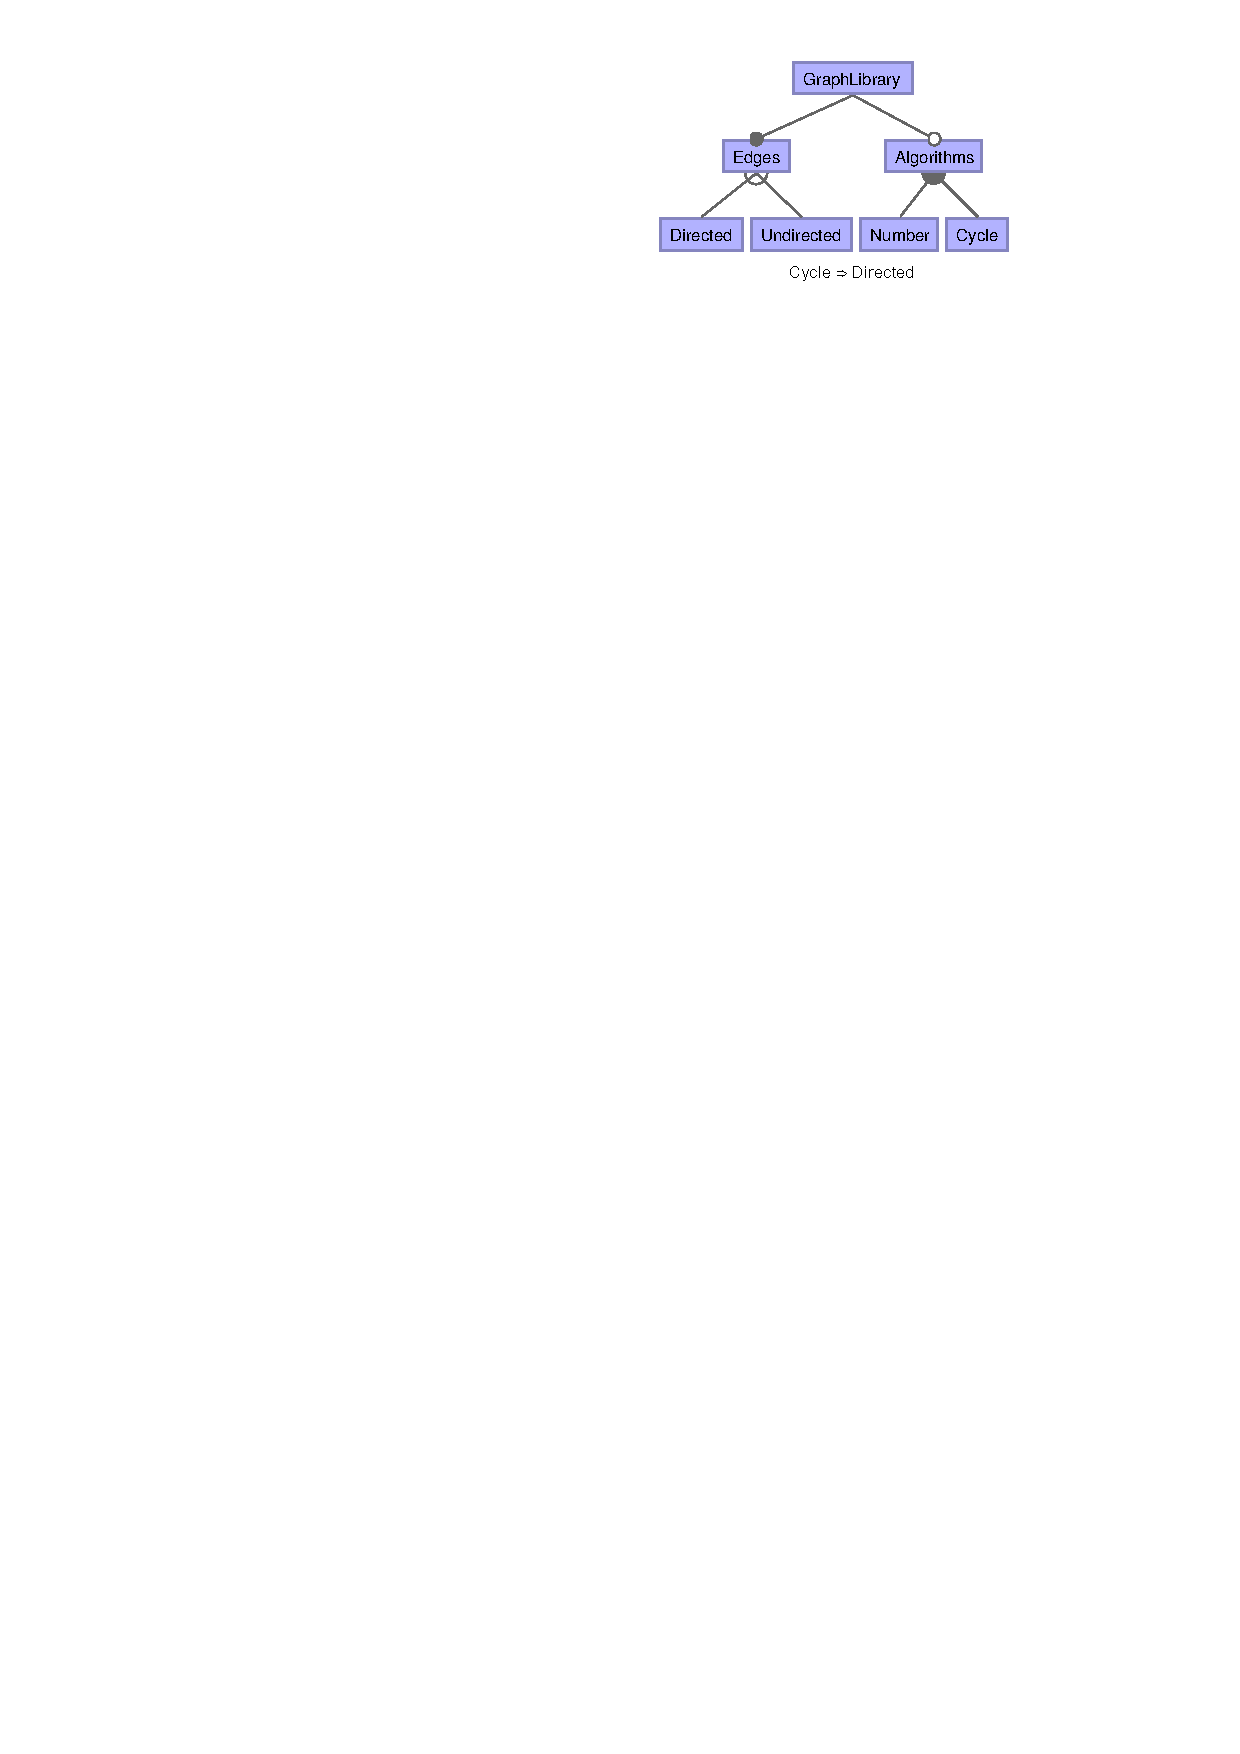
\includegraphics[scale=1.25]{example}
	\caption{A feature model representing a graph product line}
	\label{fig:ex}
\end{figure}

\section{Tables}

\vref{tab:ex} shows the result of a simple tabular environment.

\begin{table}[htbp]
	\centering
		\begin{tabular}{cc}\toprule
			Group Type & Propositional Formula\\\midrule
			And & $(P \pimplies C_{k_1} \wedge\ldots\wedge C_{k_m}) \pand (C_1\vee\ldots\vee C_n \pimplies P)$\\\addlinespace
			Or & $P \pequals C_1\vee\ldots\vee C_n$\\\addlinespace
			Alternative & $(P \pequals C_1\vee\ldots\vee C_n) \pand \mbox{atmost}1(C_1,\ldots,C_n)$\\
			\bottomrule
		\end{tabular}
	\caption{Mapping a feature model to a propositional formula}
	\label{tab:ex}
\end{table}

\section{Code Listings}

In \vref{lst:ex}, we give an example of a source code listing. 

\begin{lstlisting}[style=Java,float=htb,caption={Java source code},label={lst:ex}]
class A extends Object {
	A() { super(); }
}
class B extends Object {
	B() { super(); }
}
class Pair extends Object {
	Object fst;
	Object snd;
	Pair(Object fst, Object snd) {
		super(); this.fst=fst; this.snd=snd;
	}
	Pair setfst(Object newfst) {
		return new Pair(newfst, this.snd);
	}
}
\end{lstlisting}

\chapter{Results}
%In diesem Kapitel beschreiben Sie,
%- wie Sie versucht haben, Ihre Arbeit (z.B. Programm, Theorie, oder Algorithmus) zu verifizieren
%- Hierfür haben Sie bereits im Kapitel 3 Prognosen oder Qualitätskriterien aufgestellt, die Sie hier überprüfen
%Zu jeder zu überprüfenden Eigenschaft sollten Sie
%- ein geeignetes Experiment entwerfen, um diese Eigenschaft zu überprüfen
%- dieses Experiment beschreiben und durchführen
%- die Ergebnisse geeignet präsentieren und kommentieren

%wie lange dauert das schlussfolgern bei bestimmten veränderungen?
%wie lange für komplett unterschiedliche?



\section{Evaluation}
In this section we evaluate the correctness of all the questions asked in the interview questionnaire.
There are two ways of doing it 
  (i) By checking the answers to the questionnaire
  (ii)By Time measurements
  
\section{By checking the answers to the questionnaire}
 we check the answers given by the interviewees to the questions asked in the questionnaire. we evaluate how often a person gave correct answer to the question. we also evaluate how often a person gave wrong answer to the question. We evaluate these with respect to each question and with respect to each use case.
 
One Performance-Influence Model.
\newline
Question : Which is the most relevant Configuration option/interaction?
\newline
\newline
Use Case 1: Simple Performance-Influence Model.

\begin{table}[htb]
\centering
\caption{Simple Performance-Influence Model}
\begin{tabular}{ |c|c|c|c| } 
 \hline
 Chart Types & Radar Plot (Q 1) & Text Plot (Q 2) & Ratio Plot (Q 3) \\ 
 \hline
 Interviewee 1 & \checkmark & \checkmark & \checkmark\\
  \hline
 Interviewee 2 & \checkmark & \checkmark & \checkmark\\
  \hline
 Interviewee 3 & \checkmark & \checkmark & \times \\
  \hline
 Interviewee 4 & \checkmark & \checkmark & \checkmark\\
  \hline
 Interviewee 5 & \checkmark & \checkmark & \checkmark\\
  \hline
 Interviewee 6 & \checkmark & \checkmark & \checkmark\\
  \hline
 Interviewee 7 & \checkmark & \checkmark & \checkmark\\
  \hline
 Interviewee 8 & \checkmark & \checkmark & \checkmark\\
  \hline
 Interviewee 9 & \checkmark & \checkmark & \checkmark\\
 \hline
\end{tabular}
\end{table}

\begin{table}[htb]
\centering
\caption{Summary of above table}
\begin{tabular}{ |c|c|c|c| } 
 \hline
  Chart Types & Radar Plot (Q 1) & Text Plot (Q 2) & Ratio Plot (Q 3) \\ 
 \hline
 \% correct answer & 100\%  & 100\%  & 88.88\%\\
  \hline
 \% wrong answer & 0\% & 0\% & 11.12\%\\
  \hline
\end{tabular}
\end{table}

All the interviewees gave the correct answer to this question except one interviewee for the ratio plot.
To summarize the table in 4.1, we can answer the questions how often a person gave a correct answer and how often a person gave wrong answer to the above question for the use case - Simple Performance-Influence Model.

From the above table we can conclude that Radar or Text plot both the visualizations are equally suitable to answer this question.

Use case 2 : Complex Performance-Influence Model.

\begin{table}[htb]
\centering
\caption{Complex Performance-Influence Model}
\begin{tabular}{ |c|c|c|c| } 
 \hline
 Chart Types & Radar Plot (Q 4) & Text Plot (Q 5) & Ratio Plot (Q 6) \\ 
 \hline
 Interviewee 1 & \checkmark & \checkmark & \checkmark\\
  \hline
 Interviewee 2 & \checkmark & \checkmark & \checkmark\\
  \hline
 Interviewee 3 & \checkmark & \checkmark & \times \\
  \hline
 Interviewee 4 & \checkmark & \checkmark & \checkmark\\
  \hline
 Interviewee 5 & \checkmark & \checkmark & \times\\
  \hline
 Interviewee 6 & \checkmark & \checkmark & \checkmark\\
  \hline
 Interviewee 7 & \checkmark & \checkmark & \checkmark\\
  \hline
 Interviewee 8 & \checkmark & \checkmark & \checkmark\\
  \hline
 Interviewee 9 & \checkmark & \checkmark & \checkmark\\
 \hline
\end{tabular}
\end{table}

\begin{table}[htb]
\centering
\caption{Summary of above table}
\begin{tabular}{ |c|c|c|c| } 
 \hline
  Chart Types & Radar Plot (Q 4) & Text Plot (Q 5) & Ratio Plot (Q 6) \\ 
 \hline
 \% correct answer & 100\%  & 100\%  & 77.77\%\\
  \hline
 \% wrong answer & 0\% & 0\% & 22.23\%\\
  \hline
\end{tabular}
\end{table}

From the above tables we can conclude that to Radar Plot and Text Plot are equally suitable to answer the question asked when a complex performance-influence model is used.

Simple and Complex Performance-Influence Models:

\begin{table}[!htbp]
\centering
\caption{Summary of above table}
\begin{tabular}{ |c|c|c|c| } 
 \hline
  Chart Types & Radar Plot & Text Plot & Ratio Plot\\ 
 \hline
 \% correct answer & 100\%  & 100\%  & 83.83\%\\
  \hline
 \% wrong answer & 0\% & 0\% & 16.17\%\\
  \hline
\end{tabular}
\end{table}

From the above summary table we can conclude that for both the use cases; Simple and Complex, we can use Radar Plot or Text Plot to answer the question correctly. Ratio Plot can also be used, but it has an error rate of 16.17\%.



Question : Which is the configuration option/interaction that leads to highest performance increase and decrease?
\newline
\newline
Use Case 1: Simple Performance-Influence Model.

\begin{table}[htb]
\centering
\caption{Simple Performance-Influence Model}
\begin{tabular}{ |c|c|c|c| } 
 \hline
 Chart Types & Radar Plot (Q 7) & Text Plot (Q 8) & Ratio Plot (Q 9) \\ 
 \hline
 Interviewee 1 & \checkmark & \checkmark & \checkmark\\
  \hline
 Interviewee 2 & \times & \checkmark & \times\\
  \hline
 Interviewee 3 & \checkmark & \checkmark & \times \\
  \hline
 Interviewee 4 & \times & \checkmark & \checkmark\\
  \hline
 Interviewee 5 & \checkmark & \checkmark & \checkmark\\
  \hline
 Interviewee 6 & \checkmark & \checkmark & \checkmark\\
  \hline
 Interviewee 7 & \checkmark & \checkmark & \times \\
  \hline
 Interviewee 8 & \times & \checkmark & \checkmark\\
  \hline
 Interviewee 9 & \checkmark & \checkmark & \times\\
 \hline
\end{tabular}
\end{table}

\begin{table}[htb]
\centering
\caption{Summary of above table}
\begin{tabular}{ |c|c|c|c| } 
 \hline
  Chart Types & Radar Plot (Q 7) & Text Plot (Q 8) & Ratio Plot (Q 9) \\ 
 \hline
 \% correct answer & 70\%  & 100\%  & 60\%\\
  \hline
 \% wrong answer & 30\% & 0\% & 40\%\\
  \hline
\end{tabular}
\end{table}

From the above we can conclude that text plot is better than radar plot and ratio plot to answer this question when a simple performance-influence model is used.

Use Case 2: Complex Performance-Influence Model.

\begin{table}[htb]
\centering
\caption{Simple Performance-Influence Model}
\begin{tabular}{ |c|c|c|c| } 
 \hline
 Chart Types & Radar Plot (Q 10) & Text Plot (Q 11) \\ 
 \hline
 Interviewee 1 & \checkmark & \checkmark\\
  \hline
 Interviewee 2 & \checkmark & \checkmark\\
  \hline
 Interviewee 3 & \checkmark & \checkmark \\
  \hline
 Interviewee 4 & \checkmark & \checkmark\\
  \hline
 Interviewee 5 & \checkmark & \checkmark\\
  \hline
 Interviewee 6 & \checkmark & \checkmark\\
  \hline
 Interviewee 7 & \checkmark & \checkmark\\
  \hline
 Interviewee 8 & \checkmark & \checkmark\\
  \hline
 Interviewee 9 & \checkmark & \checkmark\\
 \hline
\end{tabular}
\end{table}

\begin{table}[!htbp]
\centering
\caption{Summary of above table}
\begin{tabular}{ |c|c|c|c| } 
 \hline
  Chart Types & Radar Plot (Q 10) & Text Plot (Q 11)\\ 
 \hline
 \% correct answer & 100\%  & 100\%\\
  \hline
 \% wrong answer & 0\% & 0\%\\
  \hline
\end{tabular}
\end{table}

We skipped the Visualization for ratio plot since it is impossible to answer this question with ratio plot.
From the above table we can conclude that radar plot and text plot are equally suitable to answer this question for a complex performance-influence model.

Simple and Complex Performance-Influence Models:

\begin{table}[htbp]
\centering
\caption{Summary of above table}
\begin{tabular}{ |c|c|c|c| } 
 \hline
  Chart Types & Radar Plot & Text Plot & Ratio Plot \\ 
 \hline
 \% correct answer & 83.34\%  & 100\%  & 60\%\\
  \hline
 \% wrong answer & 16.67\% & 0\% & 40\%\\
  \hline
\end{tabular}
\end{table}

From the above summary table we can conclude that for both the use cases; Simple and Complex, text plot can be used to answer the question correctly. Radar Plot has an error rate of 16.67\%. This question is impossible to be answer with the help of ratio plot. Hence the preferred Visualization is Text plot over radar plot.

Two Performance-Influence Models:
\newline
Question: Which is the configuration option/interaction where the performance-influence models differs the most?

Use Case 1: Simple Performance-Influence Model.

\begin{table}[htbp]
\centering
\caption{Simple Performance-Influence Model}
\begin{tabular}{ |c|c|c|c| } 
 \hline
 Chart Types & Radar Plot (Q 12) & Text Plot (Q 13) & Ratio Plot (Q 14) \\ 
 \hline
 Interviewee 1 & \checkmark & \checkmark & \checkmark\\
  \hline
 Interviewee 2 & \checkmark & \checkmark & \checkmark\\
  \hline
 Interviewee 3 & \checkmark & \checkmark & \checkmark \\
  \hline
 Interviewee 4 & \checkmark & \checkmark & \checkmark\\
  \hline
 Interviewee 5 & \checkmark & \checkmark & \checkmark\\
  \hline
 Interviewee 6 & \checkmark & \checkmark & \checkmark\\
  \hline
 Interviewee 7 & \checkmark & \checkmark & \checkmark \\
  \hline
 Interviewee 8 & \checkmark & \checkmark & \checkmark\\
  \hline
 Interviewee 9 & \checkmark & \checkmark & \checkmark\\
 \hline
\end{tabular}
\end{table}

\begin{table}[htbp]
\centering
\caption{Summary of above table}
\begin{tabular}{ |c|c|c|c| } 
 \hline
  Chart Types & Radar Plot (Q 12) & Text Plot (Q 13) & Ratio Plot (Q 14) \\ 
 \hline
 \% correct answer & 100\%  & 100\%  & 100\%\\
  \hline
 \% wrong answer & 0\% & 0\% & 0\%\\
  \hline
\end{tabular}
\end{table}

All of the interviewees gave correct answer to the question for all three visualizations. Hence any of the three visualizations can be used to answer this question when a simple performance-influence model is used.

Use Case 2 : Complex Performance-Influence Model

\begin{table}[htbp]
\centering
\caption{Complex Performance-Influence Model}
\begin{tabular}{ |c|c|c|c| } 
 \hline
 Chart Types & Radar Plot (Q 15) & Text Plot (Q 16) & Ratio Plot (Q 17) \\ 
 \hline
 Interviewee 1 & \checkmark & \checkmark & \checkmark\\
  \hline
 Interviewee 2 & \times & \checkmark & \checkmark\\
  \hline
 Interviewee 3 & \times & \checkmark & \checkmark \\
  \hline
 Interviewee 4 & \times & \checkmark & \times\\
  \hline
 Interviewee 5 & \checkmark & \checkmark & \checkmark\\
  \hline
 Interviewee 6 & \times & \checkmark & \checkmark\\
  \hline
 Interviewee 7 & \times & \checkmark & \checkmark \\
  \hline
 Interviewee 8 & \times & \checkmark & \times\\
  \hline
 Interviewee 9 & \times & \checkmark & \times\\
 \hline
\end{tabular}
\end{table}

\begin{table}[htbp]
\centering
\caption{Summary of above table}
\begin{tabular}{ |c|c|c|c| } 
 \hline
  Chart Types & Radar Plot (Q 15) & Text Plot (Q 16) & Ratio Plot (Q 17) \\ 
 \hline
 \% correct answer & 22.23\%  & 100\%  & 66.66\%\\
  \hline
 \% wrong answer & 77.78\% & 0\% & 33.34\%\\
  \hline
\end{tabular}
\end{table}

For the complex use case of the question, radar plot did not seem to be a good choice. Text plot is suitable for this question. Ratio plot also has some error rate.

\begin{table}[!htbp]
\centering
\caption{Summary of Simple and Complex Performance-Influence Model}
\begin{tabular}{ |c|c|c|c| } 
 \hline
  Chart Types & Radar Plot & Text Plot & Ratio Plot \\ 
 \hline
 \% correct answer & 61.11\%  & 100\%  & 66.66\%\\
  \hline
 \% wrong answer & 38.89\% & 0\% & 33.34\%\\
  \hline
\end{tabular}
\end{table}

From the summary of both the use cases we can conclude that Text plot is more suitable with error rate of 0\% over radar plot and ratio plot.

Question : Which is the configuration option/interaction where the performance-influence models are most similar?

Use Case 1 : Simple Performance-Influence Model

\begin{table}[!htbp]
\centering
\caption{Simple Performance-Influence Model}
\begin{tabular}{ |c|c|c|c| } 
 \hline
 Chart Types & Radar Plot (Q 18) & Text Plot (Q 19) & Ratio Plot (Q 20) \\ 
 \hline
 Interviewee 1 & \checkmark & \checkmark & \times\\
  \hline
 Interviewee 2 & \checkmark & \checkmark & \checkmark\\
  \hline
 Interviewee 3 & \checkmark & \checkmark & \times \\
  \hline
 Interviewee 4 & \checkmark & \checkmark & \times\\
  \hline
 Interviewee 5 & \checkmark & \checkmark & \checkmark\\
  \hline
 Interviewee 6 & \checkmark & \checkmark & \times\\
  \hline
 Interviewee 7 & \checkmark & \checkmark & \times \\
  \hline
 Interviewee 8 & \checkmark & \times & \times\\
  \hline
 Interviewee 9 & \checkmark & \checkmark & \times\\
 \hline
\end{tabular}
\end{table}

\begin{table}[!htbp]
\centering
\caption{Summary of above table}
\begin{tabular}{ |c|c|c|c| } 
 \hline
  Chart Types & Radar Plot (Q 18) & Text Plot (Q 19) & Ratio Plot (Q 20) \\ 
 \hline
 \% correct answer & 100\%  & 88.89\%  & 22.23\%\\
  \hline
 \% wrong answer & 0\% & 11.11\% & 77.77\%\\
  \hline
\end{tabular}
\end{table}

From the above table we can conclude that text plot is more suitable for this question than radar and ratio plot.

Use Case 2 : Complex Performance-Influence Model.

\begin{table}[!htbp]
\centering
\caption{Complex Performance-Influence Model}
\begin{tabular}{ |c|c|c|c| } 
 \hline
 Chart Types & Radar Plot (Q 21) & Text Plot (Q 22) & Ratio Plot (Q 23) \\ 
 \hline
 Interviewee 1 & \checkmark & \checkmark & \times\\
  \hline
 Interviewee 2 & \checkmark & \checkmark & \times\\
  \hline
 Interviewee 3 & \checkmark & \checkmark & \checkmark \\
  \hline
 Interviewee 4 & \checkmark & \checkmark & \checkmark\\
  \hline
 Interviewee 5 & \checkmark & \checkmark & \checkmark\\
  \hline
 Interviewee 6 & \checkmark & \checkmark & \times\\
  \hline
 Interviewee 7 & \checkmark & \checkmark & \checkmark \\
  \hline
 Interviewee 8 & \times & \times & \times\\
  \hline
 Interviewee 9 & \checkmark & \checkmark & \checkmark\\
 \hline
\end{tabular}
\end{table}

\begin{table}[!htbp]
\centering
\caption{Summary of above table}
\begin{tabular}{ |c|c|c|c| } 
 \hline
  Chart Types & Radar Plot (Q 21) & Text Plot (Q 22) & Ratio Plot (Q 23) \\ 
 \hline
 \% correct answer & 88.89\%   & 88.89\%  & 55.55\%\\
  \hline
 \% wrong answer & 11.11\% & 11.11\% & 44.45\%\\
  \hline
\end{tabular}
\end{table}

From the above table we can see that both radar plot and text plot are equally suitable to answer this question. Ratio plot has an error rate of 44.45\%.

\begin{table}[!htbp]
\centering
\caption{Summary of Simple and Complex Performance-Influence Model}
\begin{tabular}{ |c|c|c|c| } 
 \hline
  Chart Types & Radar Plot & Text Plot & Ratio Plot \\ 
 \hline
 \% correct answer & 94.45\%  & 88.89\%  & 26.66\%\\
  \hline
 \% wrong answer & 5.55\% & 11.11\% & 73.34\%\\
  \hline
\end{tabular}
\end{table}

From the summary we can see that Radar Plot is a better choice to answer this question. Text plot is the second best option, whereas ratio plot has more probability that a user would not get a correct answer to the question.

Many Performance-Influence Models

Question : Which pair of performance-influence models share a large set of influences?

\newline
Use Case 1 : Simple Performance-Influence Model

\begin{table}[!htbp]
\centering
\caption{Simple Performance-Influence Model}
\begin{tabular}{ |c|c|c|c| } 
 \hline
 Chart Types & Radar Plot (Q 24) & Text Plot (Q 25) & Ratio Plot (Q 26) \\ 
 \hline
 Interviewee 1 & \times & \checkmark & \checkmark\\
  \hline
 Interviewee 2 & \checkmark & \checkmark & \times\\
  \hline
 Interviewee 3 & \checkmark & \checkmark & \checkmark \\
  \hline
 Interviewee 4 & \checkmark & \checkmark & \checkmark\\
  \hline
 Interviewee 5 & \checkmark & \checkmark & \times\\
  \hline
 Interviewee 6 & \checkmark & \checkmark & \times\\
  \hline
 Interviewee 7 & \checkmark & \checkmark & \times \\
  \hline
 Interviewee 8 & \checkmark & \times & \times\\
  \hline
 Interviewee 9 & \checkmark & \checkmark & \times\\
 \hline
\end{tabular}
\end{table}

\begin{table}[t]
\centering
\caption{Summary of above table}
\begin{tabular}{ |c|c|c|c| } 
 \hline
  Chart Types & Radar Plot (Q 24) & Text Plot (Q 25) & Ratio Plot (Q 26) \\ 
 \hline
 \% correct answer & 88.89\%   & 88.89\%  & 33.34\%\\
  \hline
 \% wrong answer & 11.11\% & 11.11\% & 66.66\%\\
  \hline
\end{tabular}
\end{table}

From the above table we can conclude that radar plot and text plot are more suitable to answer the question than ratio plot.

Use Case 2 : Complex Performance-Influence Model

\begin{table}[!htbp]
\centering
\caption{Complex Performance-Influence Model}
\begin{tabular}{ |c|c|c|c| } 
 \hline
 Chart Types & Radar Plot (Q 27) & Text Plot (Q 28) & Ratio Plot (Q 29) \\ 
 \hline
 Interviewee 1 & \checkmark & \checkmark & \checkmark\\
  \hline
 Interviewee 2 & \times & \checkmark & \times\\
  \hline
 Interviewee 3 & \checkmark & \checkmark & \checkmark \\
  \hline
 Interviewee 4 & \checkmark & \checkmark & \checkmark\\
  \hline
 Interviewee 5 & \times & \checkmark & \checkmark\\
  \hline
 Interviewee 6 & \checkmark & \checkmark & \checkmark\\
  \hline
 Interviewee 7 & \checkmark & \checkmark & \checkmark \\
  \hline
 Interviewee 8 & \checkmark & \checkmark & \checkmark\\
  \hline
 Interviewee 9 & \times & \checkmark & \checkmark\\
 \hline
\end{tabular}
\end{table}

\begin{table}[!htbp]
\centering
\caption{Summary of above table}
\begin{tabular}{ |c|c|c|c| } 
 \hline
  Chart Types & Radar Plot (Q 27) & Text Plot (Q 28) & Ratio Plot (Q 29) \\ 
 \hline
 \% correct answer & 33.33\%   & 100\%  & 88.89\%\\
  \hline
 \% wrong answer & 66.66\% & 0\% & 11.11\%\\
  \hline
\end{tabular}
\end{table}

From the above table we can conclude that text plot is better choice to answer the question when a complex performance-influence model is used.

\begin{table}[!htbp]
\centering
\caption{Summary of Simple and Complex Performance-Influence Model}
\begin{tabular}{ |c|c|c|c| } 
 \hline
  Chart Types & Radar Plot & Text Plot & Ratio Plot \\ 
 \hline
 \% correct answer & 77.77\%  & 94.44\%  & 61.11\%\\
  \hline
 \% wrong answer & 22.22\% & 5.55\% & 38.88\%\\
  \hline
\end{tabular}
\end{table}

From the above summary table we can conclude that Text plot is more suitable to answer this question, for both simple and complex performance-influence models. Radar plot can also be used, but it might answer the question in a wrong way.

Question: Which pair of performance-influence models share a large set of influences?

Use Case 1 : Simple Performance-Influence Model


\begin{table}[!htbp]
\centering
\caption{Simple Performance-Influence Model}
\begin{tabular}{ |c|c|c|c| } 
 \hline
 Chart Types & Radar Plot (Q 30) & Text Plot (Q 31) & Ratio Plot (Q 32) \\ 
 \hline
 Interviewee 1 & \times & \times & \checkmark\\
  \hline
 Interviewee 2 & \checkmark & \times & \times\\
  \hline
 Interviewee 3 & \checkmark & \checkmark & \checkmark \\
  \hline
 Interviewee 4 & \times & \times & \checkmark\\
  \hline
 Interviewee 5 & \times & \times & \checkmark\\
  \hline
 Interviewee 6 & \checkmark & \checkmark & \checkmark\\
  \hline
 Interviewee 7 & \times & \times & \checkmark \\
  \hline
 Interviewee 8 & \times & \times & \checkmark\\
  \hline
 Interviewee 9 & \times & \times & \checkmark\\
 \hline
\end{tabular}
\end{table}

\begin{table}[!htbp]
\centering
\caption{Summary of above table}
\begin{tabular}{ |c|c|c|c| } 
 \hline
  Chart Types & Radar Plot (Q 30) & Text Plot (Q 31) & Ratio Plot (Q 32) \\ 
 \hline
 \% correct answer & 33.33\%   & 22.22\%  & 88.88\%\\
  \hline
 \% wrong answer & 66.66\% & 77.77\% & 11.11\%\\
  \hline
\end{tabular}
\end{table}

From the above table we can see that radar plot and text plot has high error rate. whereas ratio plot helps to answer this question correctly in most of the cases, while it still has an error rate of 11.11\%.

Use Case 2 : Complex Performance-Influence Model

\begin{table}[!htbp]
\centering
\caption{Complex Performance-Influence Model}
\begin{tabular}{ |c|c|c|c| } 
 \hline
 Chart Types & Radar Plot (Q 33) & Text Plot (Q 34) & Ratio Plot (Q 35) \\ 
 \hline
 Interviewee 1 & \times & \checkmark & \checkmark\\
  \hline
 Interviewee 2 & \checkmark & \checkmark & \times\\
  \hline
 Interviewee 3 & \checkmark & \checkmark & \checkmark \\
  \hline
 Interviewee 4 & \times & \times & \checkmark\\
  \hline
 Interviewee 5 & \checkmark & \checkmark & \checkmark\\
  \hline
 Interviewee 6 & \checkmark & \checkmark & \checkmark\\
  \hline
 Interviewee 7 & \times & \checkmark & \checkmark \\
  \hline
 Interviewee 8 & \times & \times & \checkmark\\
  \hline
 Interviewee 9 & \times & \checkmark & \times\\
 \hline
\end{tabular}
\end{table}

\begin{table}[!htbp]
\centering
\caption{Summary of above table}
\begin{tabular}{ |c|c|c|c| } 
 \hline
  Chart Types & Radar Plot (Q 33) & Text Plot (Q 34) & Ratio Plot (Q 35) \\ 
 \hline
 \% correct answer & 55.55\%   & 77.77\%  & 77.77\%\\
  \hline
 \% wrong answer & 44.44\% & 22.22\% & 22.22\%\\
  \hline
\end{tabular}
\end{table}

From the summary table we can see that all the visualization have an error rate, ratio plot being the more suitable one.


\begin{table}[!htbp]
\centering
\caption{Summary of Simple and Complex Performance-Influence Model}
\begin{tabular}{ |c|c|c|c| } 
 \hline
  Chart Types & Radar Plot & Text Plot & Ratio Plot \\ 
 \hline
 \% correct answer & 61.11\%  & 50\%  & 83.33\%\\
  \hline
 \% wrong answer & 38.88\% & 50\% & 16.66\%\\
  \hline
\end{tabular}
\end{table}

From the summary of both simple and complex use cases, we can conclude that ratio plot will be more suitable to answer this question than the other two visualizations since it has a lower error rate.

\ifgerman{\chapter{Verwandte Arbeiten}}{\chapter{Related Work}}
\label{relatedwork}

\todots

\ifgerman{\chapter{Zusammenfassung}}{\chapter{Conclusion}}
\label{conclusion}

Performance-influence models are used to interpret the influence of configuration options like encryption on non-functional properties like the performance of a configurable software system. With the increasing complexity of performance-influence models, it is difficult to interpret them in their original representation. Therefore, we presented different visualization techniques to ease the interpretation of performance-influence models.

We selected 3 visualization techniques; the radar plot, the text plot, and the ratio plot. To assess the quality of these visualization techniques we conducted an interview. 

Research questions were selected based on the number of performance-influence models the visualizations included. The visualizations could perform differently regarding the number of performance-influence models and, thus, we investigate how they perform with one performance-influence model, two performance-influence models, and many performance-influence models.

From the interview and their results, we found out that the text plot outperformed the radar plot and the ratio plot. The text plot presents the performance influence in a vertically aligned format and hence it is easier to perceive data than on the radar and the ratio plot. 




\ifgerman{\chapter{Zukunftige Arbeiten}}{\chapter{Future Work}}
\label{futurework}

In this section, we describe ways to improve the visualization techniques that would help the user to improve their perception of the data presented. The general feedback presented \hyperref[sec:4.6]{Section 4.6} forms as a base for our future work.

Ratio plot as we know is a visual representation of configuration options and interaction with their general performance influence on the system. It does not present the information if performance influence was positive or negative. Hence, the most of the feedback from interviewees consisted of improved ratio plot which presents if the configuration option or interaction made a positive or a negative influence on the system. One way to achieve this, is to have an axis separating positive and negative influences. \hyperref[positiveNegative]{Figure 7.1}, shows a mock-up of the same.

\begin{figure}[ht]
\centering
\label{positiveNegative}
 %- \textbf{Your title}\par\medskip
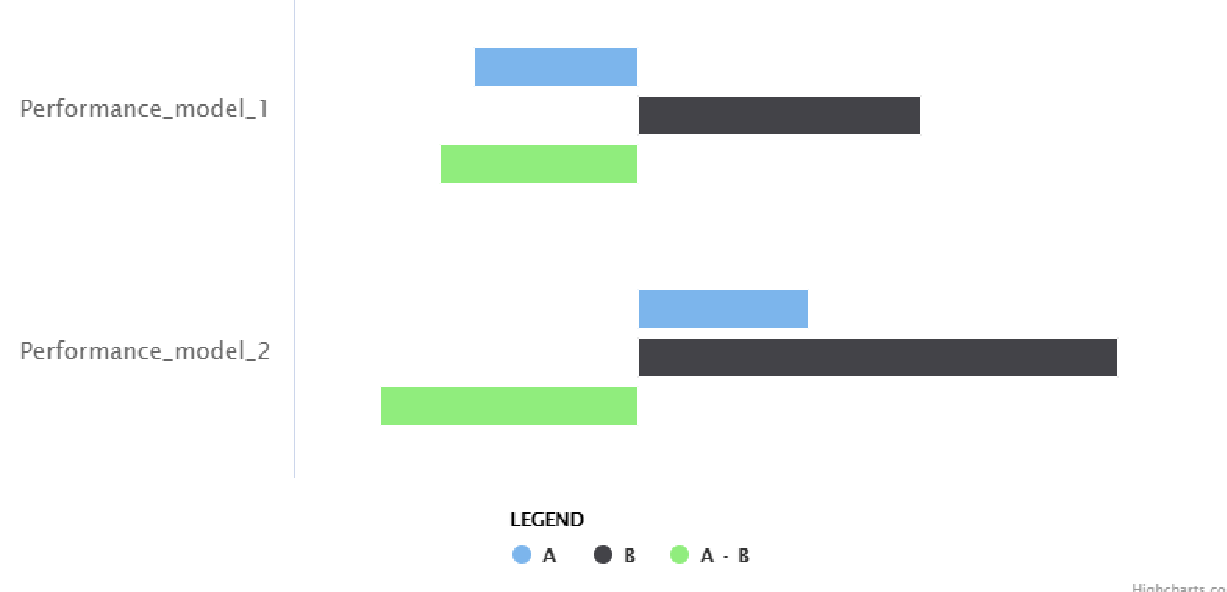
\includegraphics[width=15cm,height=15cm,keepaspectratio,]{pics/ratio_plot_with_positive_negative.pdf}
\caption[mockup1]{Mockup of ratio plot with configuration options A and B and interaction A $\cdot$ B for two performance-influence models, with separation between negative influences to the left side and positive influences to the right side of the center axis}
\end{figure}

Another improvement on ratio plot would be to show all the configuration options and interactions in the same order for all the performance-influence models. Currently, we display the configuration options and interactions in a sorted order from highest to lowest performance influence for each performance-influence model, which makes comparison a difficult task.  \hyperref[sameOrder]{Figure 7.2}, is a mock-up of the same.

\begin{figure}[ht]
\centering
\label{sameOrder}
 %- \textbf{Your title}\par\medskip
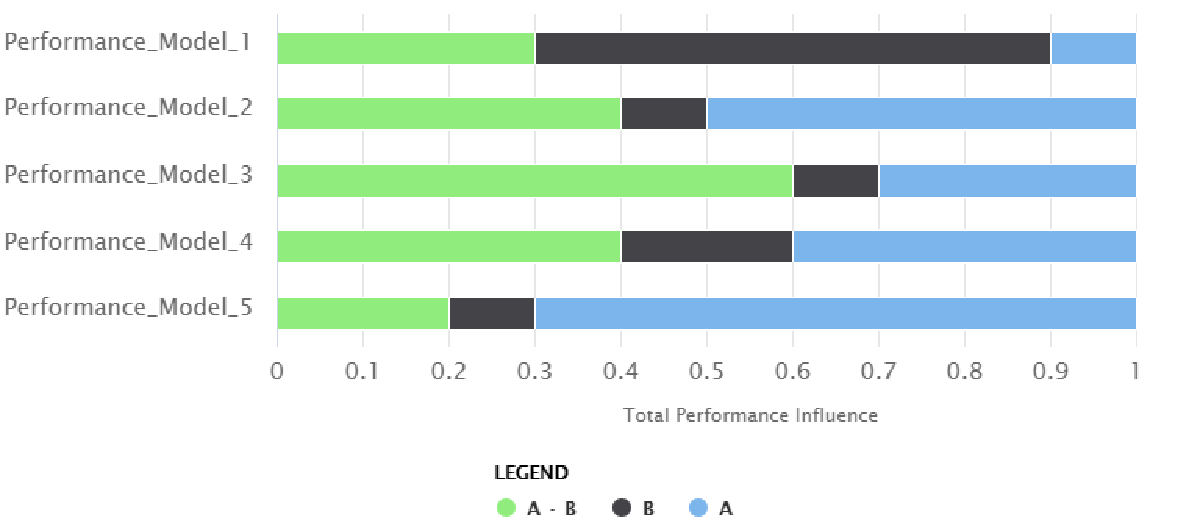
\includegraphics[width=15cm,height=15cm,keepaspectratio,]{pics/ratio_plot_without_sorted_order.pdf}
\caption[mockup2]{Mockup of ratio plot with configuration options A and B and interaction A $\cdot$ B of 5 performance-influence models all displayed in the same order}
\end{figure}


An improvement suggested for radar and text plot was to present the configuration options and interactions in a sorted order. This would help the users perception in finding the most relevant configuration option or interaction easily.



%*********************************************************************%
% APPENDIX                                                             %
%*********************************************************************%

\appendix
\ifgerman{\chapter{Anhang}}{\chapter{Appendix}}
\label{appedixa}

\section{Difficulty Rating vs Time measurements co-relation}
\label{sanityCheck}
Sanity check is made to ensure that the assumption made from the results of difficulty rating hold true. To conduct the sanity check, we plot graphs with difficulty rating against time taken to answer a question, per interviewee.

\begin{figure}[H]
\centering
\begin{adjustbox}{width=1\textwidth}
\begin{minipage}[8cm]{.44\textwidth}
\begin{tikzpicture}[scale=0.80]
	\begin{axis}[%
	xlabel={Difficulty Ratings},
    ylabel={Time(in seconds)},
    ymin=0,
    minor y tick num=2,
    grid style={dashed,gray!30},
    ymajorgrids=true,
    xmajorgrids=true,
    yminorgrids=true,
    only marks,
    scatter,
    mark size=3.5pt,
    scatter src=explicit symbolic,
	scatter/classes={
		a={mark=square,draw=gray},
		b={mark=triangle,draw=gray},
		c={mark=otimes,draw=gray},
		x={mark=diamond,draw=gray},
	    y={mark=oplus,draw=gray},
		z={mark=star,draw=gray},
		q1sRa={mark=square,draw=green},
	    q1sT={mark=triangle,draw=green},
		q1sRo={mark=otimes,draw=green},
		q1cRa={mark=diamond,draw=green},
	    q1cT={mark=oplus,draw=green},
		q1cRo={mark=star,draw=green},
		q2sRa={mark=square,draw=orange},
	    q2sT={mark=triangle,draw=orange},
		q2sRo={mark=otimes,draw=orange},
		q2cRa={mark=diamond,draw=orange},
	    q2cT={mark=oplus,draw=orange},
		q2cRo={mark=star,draw=orange},
		q3sRa={mark=square,draw=blue},
	    q3sT={mark=triangle,draw=blue},
		q3sRo={mark=otimes,draw=blue},
		q3cRa={mark=diamond,draw=blue},
	    q3cT={mark=oplus,draw=blue},
		q3cRo={mark=star,draw=blue},
		q4sRa={mark=square,draw=red},
	    q4sT={mark=triangle,draw=red},
		q4sRo={mark=otimes,draw=red},
		q4cRa={mark=diamond,draw=red},
	    q4cT={mark=oplus,draw=red},
		q4cRo={mark=star,draw=red},
		q5sRa={mark=square,draw=black},
	    q5sT={mark=triangle,draw=black},
		q5sRo={mark=otimes,draw=black},
		q5cRa={mark=diamond,draw=black},
	    q5cT={mark=oplus,draw=black},
		q5cRo={mark=star,draw=black},
		q6sRa={mark=square,draw=cyan},
	    q6sT={mark=triangle,draw=cyan},
		q6sRo={mark=otimes,draw=cyan},
		q6cRa={mark=diamond,draw=cyan},
	    q6cT={mark=oplus,draw=cyan},
		q6cRo={mark=star,draw=cyan}},]
	\addplot[scatter,only marks,%
		scatter src=explicit symbolic]%
	table[meta=label] {
x         y         label
2	11.21	q1sRa
2	10.679	q1sT
1	13.292	q1sRo
		
3	30.59	q1cRa
3	25.252	q1cT
1	26.866	q1cRo
		
		
2	44.209	q2sRa
1	27.535	q2sT
5	70.4	q2sRo
		
3	39.415	q2cRa
3	32.897	q2cT
		
		
2	13.983	q3sRa
2	15.166	q3sT
5	34.07	q3sRo
		
4	53.26	q3cRa
2	23.036	q3cT
3	61.0	q3cRo
		
		
19

1	12.843	q4sRa
2	15.801	q4sT
4	32.092	q4sRo
		
2	28.282	q4cRa
2	30.629	q4cT
3	334.0	q4cRo
		
		
5	70.056	q5sRa
2	132.19	q5sT
4   110	    q5sRo
		
3	24.874	q5cRa
2	41.139	q5cT
4	68.315	q5cRo
		
		
2	102.026	q6sRa
4	32.672	q6sT
3	47.104	q6sRo
		
2	20.264	q6cRa
2	54.906	q6cT
5	55.942	q6cRo
};
\end{axis}
\begin{axis}[
    xmin=0,
    xmax=100,
    ymin=1,
    ymax=6,
    hide axis,
    only marks,
    ]
\foreach \i in {0,...,6} {
        \addplot+ [mark=*] coordinates { (0,0) };
     }
    \end{axis}
\end{tikzpicture}
\caption{Difficulty rating and time measurements for interviewee 1}\label{figure:interviewee1}
\vspace{\baselineskip}
\end{minipage}
\begin{minipage}[8cm]{.44\textwidth}
\begin{tikzpicture}[scale=0.80]
	\begin{axis}[%
	xlabel={Difficulty Ratings},
    ylabel={Time(in seconds)},
    ymin=0,
    minor y tick num=2,
    grid style={dashed,gray!30},
    ymajorgrids=true,
    xmajorgrids=true,
    yminorgrids=true,
    only marks,
    scatter,
    mark size=3.5pt,
    scatter src=explicit symbolic,
	scatter/classes={
		a={mark=square,draw=gray},
		b={mark=triangle,draw=gray},
		c={mark=otimes,draw=gray},
		x={mark=diamond,draw=gray},
	    y={mark=oplus,draw=gray},
		z={mark=star,draw=gray},
		q1sRa={mark=square,draw=green},
	    q1sT={mark=triangle,draw=green},
		q1sRo={mark=otimes,draw=green},
		q1cRa={mark=diamond,draw=green},
	    q1cT={mark=oplus,draw=green},
		q1cRo={mark=star,draw=green},
		q2sRa={mark=square,draw=orange},
	    q2sT={mark=triangle,draw=orange},
		q2sRo={mark=otimes,draw=orange},
		q2cRa={mark=diamond,draw=orange},
	    q2cT={mark=oplus,draw=orange},
		q2cRo={mark=star,draw=orange},
		q3sRa={mark=square,draw=blue},
	    q3sT={mark=triangle,draw=blue},
		q3sRo={mark=otimes,draw=blue},
		q3cRa={mark=diamond,draw=blue},
	    q3cT={mark=oplus,draw=blue},
		q3cRo={mark=star,draw=blue},
		q4sRa={mark=square,draw=red},
	    q4sT={mark=triangle,draw=red},
		q4sRo={mark=otimes,draw=red},
		q4cRa={mark=diamond,draw=red},
	    q4cT={mark=oplus,draw=red},
		q4cRo={mark=star,draw=red},
		q5sRa={mark=square,draw=black},
	    q5sT={mark=triangle,draw=black},
		q5sRo={mark=otimes,draw=black},
		q5cRa={mark=diamond,draw=black},
	    q5cT={mark=oplus,draw=black},
		q5cRo={mark=star,draw=black},
		q6sRa={mark=square,draw=cyan},
	    q6sT={mark=triangle,draw=cyan},
		q6sRo={mark=otimes,draw=cyan},
		q6cRa={mark=diamond,draw=cyan},
	    q6cT={mark=oplus,draw=cyan},
		q6cRo={mark=star,draw=cyan}}]
	\addplot[scatter,only marks,%
		scatter src=explicit symbolic]%
	table[meta=label] {
x         y         label
		
		
1	10.2	q1sRa
1	3.23	q1sT
1	10.45	q1sRo
		
2	10.12	q1cRa
2	7.02	q1cT
2	14.33	q1cRo
		
		
2	22.27	q2sRa
3	16.11	q2sT
3	30.6	q2sRo
		
2	32.19	q2cRa
2	21.49	q2cT
		
		
2	21.64	q3sRa
2	6	q3sT
2	20.43	q3sRo
		
2	19.82	q3cRa
2	14.88	q3cT
2	21.84	q3cRo
		
		
2	9.07	q4sRa
2	7.04	q4sT
3	24.2	q4sRo
		
3	21.71	q4cRa
2	15.53	q4cT
4	35.03	q4cRo
		
		
3	43.14	q5sRa
2	25.58	q5sT
5	73.39	q5sRo
		
4	52.97	q5cRa
1	24.97	q5cT
5	6.33	q5cRo
		
		
4	41.64	q6sRa
4	65.88	q6sT
5	11.25	q6sRo
		
2	29.91	q6cRa
2	19.16	q6cT
5	14.82	q6cRo

};
\end{axis}
	
\begin{axis}[
    xmin=0,
    xmax=100,
    ymin=1,
    ymax=6,
    hide axis,
    only marks,
    ]
\foreach \i in {0,...,6} {
        \addplot+ [mark=*] coordinates { (0,0) };
     }
    \end{axis}
\end{tikzpicture}
\caption{Difficulty rating and time measurements for interviewee 2} 
\label{figure:interviewee2}
\vspace{\baselineskip}
\end{minipage}



\end{adjustbox}
\end{figure}

\begin{figure}[H]
\centering
\begin{adjustbox}{width=1\textwidth}
\begin{minipage}[8cm]{.44\textwidth}
\begin{tikzpicture}[scale=0.80]
	\begin{axis}[%
	xlabel={Difficulty Ratings},
    ylabel={Time(in seconds)},
    ymin=0,
    minor y tick num=2,
    grid style={dashed,gray!30},
    ymajorgrids=true,
    xmajorgrids=true,
    yminorgrids=true,
    only marks,
    scatter,
    mark size=3.5pt,
    scatter src=explicit symbolic,
	scatter/classes={
		a={mark=square,draw=gray},
		b={mark=triangle,draw=gray},
		c={mark=otimes,draw=gray},
		x={mark=diamond,draw=gray},
	    y={mark=oplus,draw=gray},
		z={mark=star,draw=gray},
		q1sRa={mark=square,draw=green},
	    q1sT={mark=triangle,draw=green},
		q1sRo={mark=otimes,draw=green},
		q1cRa={mark=diamond,draw=green},
	    q1cT={mark=oplus,draw=green},
		q1cRo={mark=star,draw=green},
		q2sRa={mark=square,draw=orange},
	    q2sT={mark=triangle,draw=orange},
		q2sRo={mark=otimes,draw=orange},
		q2cRa={mark=diamond,draw=orange},
	    q2cT={mark=oplus,draw=orange},
		q2cRo={mark=star,draw=orange},
		q3sRa={mark=square,draw=blue},
	    q3sT={mark=triangle,draw=blue},
		q3sRo={mark=otimes,draw=blue},
		q3cRa={mark=diamond,draw=blue},
	    q3cT={mark=oplus,draw=blue},
		q3cRo={mark=star,draw=blue},
		q4sRa={mark=square,draw=red},
	    q4sT={mark=triangle,draw=red},
		q4sRo={mark=otimes,draw=red},
		q4cRa={mark=diamond,draw=red},
	    q4cT={mark=oplus,draw=red},
		q4cRo={mark=star,draw=red},
		q5sRa={mark=square,draw=black},
	    q5sT={mark=triangle,draw=black},
		q5sRo={mark=otimes,draw=black},
		q5cRa={mark=diamond,draw=black},
	    q5cT={mark=oplus,draw=black},
		q5cRo={mark=star,draw=black},
		q6sRa={mark=square,draw=cyan},
	    q6sT={mark=triangle,draw=cyan},
		q6sRo={mark=otimes,draw=cyan},
		q6cRa={mark=diamond,draw=cyan},
	    q6cT={mark=oplus,draw=cyan},
		q6cRo={mark=star,draw=cyan}},]
	\addplot[scatter,only marks,%
		scatter src=explicit symbolic]%
	table[meta=label] {
x         y         label
2	5.024	q1sRa
2	10.598	q1sT
1	8.192	q1sRo
		
3	17.776	q1cRa
2	24.036	q1cT
1	13.924	q1cRo
		
		
3	28.976	q2sRa
3	22.55	q2sT
4	71.008	q2sRo
		
2	30.775	q2cRa
2	28.218	q2cT
		
		
2	21.04	q3sRa
2	26.556	q3sT
5	144.0	q3sRo
		
3	69.0	q3cRa
2	28.73	q3cT
3	35.122	q3cRo
		
		
2	28.97	q4sRa
2	31.51	q4sT
5	139.0	q4sRo
		
3	26.741	q4cRa
2	28.969	q4cT
3	72.741	q4cRo
		
		
3	85.5	q5sRa
4	99.7	q5sT
5	313.555	q5sRo
		
4	171.4	q5cRa
3	196.8	q5cT
5	146.903	q5cRo
		
		
3	49.043	q6sRa
3	110.686	q6sT
5	159.1	q6sRo
		
3	51.01	q6cRa
3	40.757	q6cT
5	288.940	q6cRo
};
\end{axis}
	
\begin{axis}[
    xmin=0,
    xmax=100,
    ymin=1,
    ymax=6,
    hide axis,
    only marks,
    ]
\foreach \i in {0,...,6} {
        \addplot+ [mark=*] coordinates { (0,0) };
     }
    \end{axis}
\end{tikzpicture}
\caption{Difficulty rating and time measurements for interviewee 3}\label{figure:interviewee3}
\vspace{\baselineskip}
\end{minipage}
\begin{minipage}[8cm]{.44\textwidth}
\begin{tikzpicture}[scale=0.80]
	\begin{axis}[%
	xlabel={Difficulty Ratings},
    ylabel={Time(in seconds)},
    ymin=0,
    minor y tick num=2,
    grid style={dashed,gray!30},
    ymajorgrids=true,
    xmajorgrids=true,
    yminorgrids=true,
    only marks,
    scatter,
    mark size=3.5pt,
    scatter src=explicit symbolic,
	scatter/classes={
		a={mark=square,draw=gray},
		b={mark=triangle,draw=gray},
		c={mark=otimes,draw=gray},
		x={mark=diamond,draw=gray},
	    y={mark=oplus,draw=gray},
		z={mark=star,draw=gray},
		q1sRa={mark=square,draw=green},
	    q1sT={mark=triangle,draw=green},
		q1sRo={mark=otimes,draw=green},
		q1cRa={mark=diamond,draw=green},
	    q1cT={mark=oplus,draw=green},
		q1cRo={mark=star,draw=green},
		q2sRa={mark=square,draw=orange},
	    q2sT={mark=triangle,draw=orange},
		q2sRo={mark=otimes,draw=orange},
		q2cRa={mark=diamond,draw=orange},
	    q2cT={mark=oplus,draw=orange},
		q2cRo={mark=star,draw=orange},
		q3sRa={mark=square,draw=blue},
	    q3sT={mark=triangle,draw=blue},
		q3sRo={mark=otimes,draw=blue},
		q3cRa={mark=diamond,draw=blue},
	    q3cT={mark=oplus,draw=blue},
		q3cRo={mark=star,draw=blue},
		q4sRa={mark=square,draw=red},
	    q4sT={mark=triangle,draw=red},
		q4sRo={mark=otimes,draw=red},
		q4cRa={mark=diamond,draw=red},
	    q4cT={mark=oplus,draw=red},
		q4cRo={mark=star,draw=red},
		q5sRa={mark=square,draw=black},
	    q5sT={mark=triangle,draw=black},
		q5sRo={mark=otimes,draw=black},
		q5cRa={mark=diamond,draw=black},
	    q5cT={mark=oplus,draw=black},
		q5cRo={mark=star,draw=black},
		q6sRa={mark=square,draw=cyan},
	    q6sT={mark=triangle,draw=cyan},
		q6sRo={mark=otimes,draw=cyan},
		q6cRa={mark=diamond,draw=cyan},
	    q6cT={mark=oplus,draw=cyan},
		q6cRo={mark=star,draw=cyan}},]
	\addplot[scatter,only marks,%
		scatter src=explicit symbolic]%
	table[meta=label] {
x         y         label
		
		
1	20.089	q1sRa
1	24.125	q1sT
2	20.362	q1sRo
		
1	6.124	q1cRa
1	10.416	q1cT
1	31.608	q1cRo
		
		
1	14.328	q2sRa
1	30.085	q2sT
5	15.913	q2sRo
		
1	14.296	q2cRa
2	29.725	q2cT
		
		
1	2.357	q3sRa
1	12.884	q3sT
4	11.979	q3sRo
		
5	20.154	q3cRa
2	7.927	q3cT
5	21.694	q3cRo
		
		
2	24.296	q4sRa
2	45.527	q4sT
4	91.9	q4sRo
		
2	25.298	q4cRa
2	35.165	q4cT
3	46.726	q4cRo
		
		
3	125.0	q5sRa
2	36.758	q5sT
5	45.017	q5sRo
		
2	13.229	q5cRa
2	24.62	q5cT
5	27.879	q5cRo
		
		
3	45.44	q6sRa
3	53.34	q6sT
4	68.346	q6sRo
		
2	54.65	q6cRa
2	34.56	q6cT
4	65.34	q6cRo

};
\end{axis}
	
\begin{axis}[
    xmin=0,
    xmax=100,
    ymin=1,
    ymax=6,
    hide axis,
    only marks,]
\foreach \i in {0,...,6} {
        \addplot+ [mark=*] coordinates { (0,0) };
     }
    \end{axis}
\end{tikzpicture}
\caption{Difficulty rating and time measurements for interviewee 4}\label{figure:interviewee4}
\vspace{\baselineskip}
\end{minipage}
\end{adjustbox}
\end{figure}

\begin{figure}[H]
\centering
\begin{adjustbox}{width=1\textwidth}
\begin{minipage}[8cm]{.44\textwidth}
\begin{tikzpicture}[scale=0.80]
	\begin{axis}[%
	xlabel={Difficulty Ratings},
    ylabel={Time(in seconds)},
    ymin=0,
    minor y tick num=2,
    grid style={dashed,gray!30},
    ymajorgrids=true,
    xmajorgrids=true,
    yminorgrids=true,
    only marks,
    scatter,
    mark size=3.5pt,
    scatter src=explicit symbolic,
	scatter/classes={
		a={mark=square,draw=gray},
		b={mark=triangle,draw=gray},
		c={mark=otimes,draw=gray},
		x={mark=diamond,draw=gray},
	    y={mark=oplus,draw=gray},
		z={mark=star,draw=gray},
		q1sRa={mark=square,draw=green},
	    q1sT={mark=triangle,draw=green},
		q1sRo={mark=otimes,draw=green},
		q1cRa={mark=diamond,draw=green},
	    q1cT={mark=oplus,draw=green},
		q1cRo={mark=star,draw=green},
		q2sRa={mark=square,draw=orange},
	    q2sT={mark=triangle,draw=orange},
		q2sRo={mark=otimes,draw=orange},
		q2cRa={mark=diamond,draw=orange},
	    q2cT={mark=oplus,draw=orange},
		q2cRo={mark=star,draw=orange},
		q3sRa={mark=square,draw=blue},
	    q3sT={mark=triangle,draw=blue},
		q3sRo={mark=otimes,draw=blue},
		q3cRa={mark=diamond,draw=blue},
	    q3cT={mark=oplus,draw=blue},
		q3cRo={mark=star,draw=blue},
		q4sRa={mark=square,draw=red},
	    q4sT={mark=triangle,draw=red},
		q4sRo={mark=otimes,draw=red},
		q4cRa={mark=diamond,draw=red},
	    q4cT={mark=oplus,draw=red},
		q4cRo={mark=star,draw=red},
		q5sRa={mark=square,draw=black},
	    q5sT={mark=triangle,draw=black},
		q5sRo={mark=otimes,draw=black},
		q5cRa={mark=diamond,draw=black},
	    q5cT={mark=oplus,draw=black},
		q5cRo={mark=star,draw=black},
		q6sRa={mark=square,draw=cyan},
	    q6sT={mark=triangle,draw=cyan},
		q6sRo={mark=otimes,draw=cyan},
		q6cRa={mark=diamond,draw=cyan},
	    q6cT={mark=oplus,draw=cyan},
		q6cRo={mark=star,draw=cyan}},]
	\addplot[scatter,only marks,%
		scatter src=explicit symbolic]%
	table[meta=label] {
x         y         label
1	33.57	q1sRa
2	23.46	q1sT
1	11.93	q1sRo
		
3	10.01	q1cRa
3	17.28	q1cT
2	15.46	q1cRo
		
		
1	30.98	q2sRa
1	13.76	q2sT
5	24.32	q2sRo
		
2	34.1	q2cRa
2	24.4	q2cT
		
		
2	30.68	q3sRa
2	7.45	q3sT
3	25.5	q3sRo
		
3	37.88	q3cRa
2	22.25	q3cT
3	54.98	q3cRo
		
		
2	15.45	q4sRa
1	10.9	q4sT
4	35.67	q4sRo
		
3	23.11	q4cRa
2	18.29	q4cT
5	60.23	q4cRo
		
		
3	146.31	q5sRa
3	56.9	q5sT
5	66.84	q5sRo
		
3	122.44	q5cRa
2	58.59	q5cT
5	40.88	q5cRo
		
		
3	74.57	q6sRa
3	38.44	q6sT
3	43.02	q6sRo
		
3	57.25	q6cRa
2	26.93	q6cT
4	83.55	q6cRo


};
\end{axis}
	
\begin{axis}[
    xmin=0,
    xmax=100,
    ymin=1,
    ymax=6,
    hide axis,
    only marks,
    ]
\foreach \i in {0,...,6} {
        \addplot+ [mark=*] coordinates { (0,0) };
     }
    \end{axis}
\end{tikzpicture}
\caption{Difficulty rating and time measurements for interviewee 5}\label{figure:interviewee5}
\vspace{\baselineskip}
\end{minipage}
\begin{minipage}[8cm]{.44\textwidth}
\begin{tikzpicture}[scale=0.80]
	\begin{axis}[%
	xlabel={Difficulty Ratings},
    ylabel={Time(in seconds)},
    ymin=0,
    minor y tick num=2,
    grid style={dashed,gray!30},
    ymajorgrids=true,
    xmajorgrids=true,
    yminorgrids=true,
    only marks,
    scatter,
    mark size=3.5pt,
    scatter src=explicit symbolic,
	scatter/classes={
		a={mark=square,draw=gray},
		b={mark=triangle,draw=gray},
		c={mark=otimes,draw=gray},
		x={mark=diamond,draw=gray},
	    y={mark=oplus,draw=gray},
		z={mark=star,draw=gray},
		q1sRa={mark=square,draw=green},
	    q1sT={mark=triangle,draw=green},
		q1sRo={mark=otimes,draw=green},
		q1cRa={mark=diamond,draw=green},
	    q1cT={mark=oplus,draw=green},
		q1cRo={mark=star,draw=green},
		q2sRa={mark=square,draw=orange},
	    q2sT={mark=triangle,draw=orange},
		q2sRo={mark=otimes,draw=orange},
		q2cRa={mark=diamond,draw=orange},
	    q2cT={mark=oplus,draw=orange},
		q2cRo={mark=star,draw=orange},
		q3sRa={mark=square,draw=blue},
	    q3sT={mark=triangle,draw=blue},
		q3sRo={mark=otimes,draw=blue},
		q3cRa={mark=diamond,draw=blue},
	    q3cT={mark=oplus,draw=blue},
		q3cRo={mark=star,draw=blue},
		q4sRa={mark=square,draw=red},
	    q4sT={mark=triangle,draw=red},
		q4sRo={mark=otimes,draw=red},
		q4cRa={mark=diamond,draw=red},
	    q4cT={mark=oplus,draw=red},
		q4cRo={mark=star,draw=red},
		q5sRa={mark=square,draw=black},
	    q5sT={mark=triangle,draw=black},
		q5sRo={mark=otimes,draw=black},
		q5cRa={mark=diamond,draw=black},
	    q5cT={mark=oplus,draw=black},
		q5cRo={mark=star,draw=black},
		q6sRa={mark=square,draw=cyan},
	    q6sT={mark=triangle,draw=cyan},
		q6sRo={mark=otimes,draw=cyan},
		q6cRa={mark=diamond,draw=cyan},
	    q6cT={mark=oplus,draw=cyan},
		q6cRo={mark=star,draw=cyan}}]
	\addplot[scatter,only marks,%
		scatter src=explicit symbolic]%
	table[meta=label] {
x         y         label
2	36.969	q1sRa
2	22.17	q1sT
1	16.967	q1sRo
		
2	24.232	q1cRa
3	32.167	q1cT
1	33.992	q1cRo
		
		
2	34.977	q2sRa
2	25.743	q2sT
2	43.967	q2sRo
		
2	18.869	q2cRa
2	36.871	q2cT
		
		
2	20.768	q3sRa
1	12.771	q3sT
3	29.559	q3sRo
		
1	13.532	q3cRa
2	16.686	q3cT
4	44.234	q3cRo
		
		
2	22.515	q4sRa
2	13.725	q4sT
3	33.804	q4sRo
		
3	25.71	q4cRa
2	24.5	q4cT
3	25.446	q4cRo
		
		
2	 67.798	q5sRa
2	40.329	q5sT
4	 76.052	q5sRo
		
2	21.658	q5cRa
2	54.374	q5cT
4	46.601	q5cRo
		
3	33.894	q6sRa
3	59.25	q6sT
5	715.016	q6sRo
		
2	55.654	q6cRa
2	39.917	q6cT
5	52.343	q6cRo
};
\end{axis}
	
\begin{axis}[
    xmin=0,
    xmax=100,
    ymin=1,
    ymax=6,
    hide axis,
    only marks,
    ]
\foreach \i in {0,...,6} {
        \addplot+ [mark=*] coordinates { (0,0) };
     }
    \end{axis}
\end{tikzpicture}
\caption{Difficulty rating and time measurements for interviewee 6}\label{figure:interviewee6}
\vspace{\baselineskip}
\end{minipage}
\end{adjustbox}
\end{figure}

\begin{figure}[H]
\centering
\begin{adjustbox}{width=1\textwidth}
\begin{minipage}[8cm]{.44\textwidth}
\begin{tikzpicture}[scale=0.80]
	\begin{axis}[%
	xlabel={Difficulty Ratings},
    ylabel={Time(in seconds)},
    ymin=0,
    minor y tick num=2,
    grid style={dashed,gray!30},
    ymajorgrids=true,
    xmajorgrids=true,
    yminorgrids=true,
    only marks,
    scatter,
    mark size=3.5pt,
    scatter src=explicit symbolic,
	scatter/classes={
		a={mark=square,draw=gray},
		b={mark=triangle,draw=gray},
		c={mark=otimes,draw=gray},
		x={mark=diamond,draw=gray},
	    y={mark=oplus,draw=gray},
		z={mark=star,draw=gray},
		q1sRa={mark=square,draw=green},
	    q1sT={mark=triangle,draw=green},
		q1sRo={mark=otimes,draw=green},
		q1cRa={mark=diamond,draw=green},
	    q1cT={mark=oplus,draw=green},
		q1cRo={mark=star,draw=green},
		q2sRa={mark=square,draw=orange},
	    q2sT={mark=triangle,draw=orange},
		q2sRo={mark=otimes,draw=orange},
		q2cRa={mark=diamond,draw=orange},
	    q2cT={mark=oplus,draw=orange},
		q2cRo={mark=star,draw=orange},
		q3sRa={mark=square,draw=blue},
	    q3sT={mark=triangle,draw=blue},
		q3sRo={mark=otimes,draw=blue},
		q3cRa={mark=diamond,draw=blue},
	    q3cT={mark=oplus,draw=blue},
		q3cRo={mark=star,draw=blue},
		q4sRa={mark=square,draw=red},
	    q4sT={mark=triangle,draw=red},
		q4sRo={mark=otimes,draw=red},
		q4cRa={mark=diamond,draw=red},
	    q4cT={mark=oplus,draw=red},
		q4cRo={mark=star,draw=red},
		q5sRa={mark=square,draw=black},
	    q5sT={mark=triangle,draw=black},
		q5sRo={mark=otimes,draw=black},
		q5cRa={mark=diamond,draw=black},
	    q5cT={mark=oplus,draw=black},
		q5cRo={mark=star,draw=black},
		q6sRa={mark=square,draw=cyan},
	    q6sT={mark=triangle,draw=cyan},
		q6sRo={mark=otimes,draw=cyan},
		q6cRa={mark=diamond,draw=cyan},
	    q6cT={mark=oplus,draw=cyan},
		q6cRo={mark=star,draw=cyan}},]
	\addplot[scatter,only marks,%
		scatter src=explicit symbolic]%
	table[meta=label] {
x         y         label
1	23.266	q1sRa
1	12.262	q1sT
1	18.282	q1sRo
		
2	39.292	q1cRa
2	16.376	q1cT
1	26.229	q1cRo
		
		
1	25.712	q2sRa
1	14.18	q2sT
5	42.934	q2sRo
		
2	26.911	q2cRa
2	22.574	q2cT
		
		
1	10.217	q3sRa
1	9.968	q3sT
1	30.947	q3sRo
		
2	56.401	q3cRa
2	12.044	q3cT
2	39.93	q3cRo
		
		
1	7.731	q4sRa
2	22.087	q4sT
2	27.443	q4sRo
		
2	26.379	q4cRa
2	9.274	q4cT
2	63.0	q4cRo
		
		
1	56.019	q5sRa
1	25.968	q5sT
4	97.1	q5sRo
		
1	18.88	q5cRa
1	25.893	q5cT
3	69.359	q5cRo
		
		
2	17.963	q6sRa
2	41.166	q6sT
2	27.851	q6sRo
		
2	17.708	q6cRa
2	17.255	q6cT
3	5.981	q6cRo

};
\end{axis}
	
\begin{axis}[
    xmin=0,
    xmax=100,
    ymin=1,
    ymax=6,
    hide axis,
    only marks,
    ]
\foreach \i in {0,...,6} {
        \addplot+ [mark=*] coordinates { (0,0) };
     }
    \end{axis}
\end{tikzpicture}
\caption{Difficulty rating and time measurements for interviewee 7}\label{figure:interviewee7}
\vspace{\baselineskip}
\end{minipage}
\begin{minipage}[8cm]{.44\textwidth}
\begin{tikzpicture}[scale=0.80]
	\begin{axis}[%
	xlabel={Difficulty Ratings},
    ylabel={Time(in seconds)},
    ymin=0,
    minor y tick num=2,
    grid style={dashed,gray!30},
    ymajorgrids=true,
    xmajorgrids=true,
    yminorgrids=true,
    only marks,
    scatter,
    mark size=3.5pt,
    scatter src=explicit symbolic,
	scatter/classes={
		a={mark=square,draw=gray},
		b={mark=triangle,draw=gray},
		c={mark=otimes,draw=gray},
		x={mark=diamond,draw=gray},
	    y={mark=oplus,draw=gray},
		z={mark=star,draw=gray},
		q1sRa={mark=square,draw=green},
	    q1sT={mark=triangle,draw=green},
		q1sRo={mark=otimes,draw=green},
		q1cRa={mark=diamond,draw=green},
	    q1cT={mark=oplus,draw=green},
		q1cRo={mark=star,draw=green},
		q2sRa={mark=square,draw=orange},
	    q2sT={mark=triangle,draw=orange},
		q2sRo={mark=otimes,draw=orange},
		q2cRa={mark=diamond,draw=orange},
	    q2cT={mark=oplus,draw=orange},
		q2cRo={mark=star,draw=orange},
		q3sRa={mark=square,draw=blue},
	    q3sT={mark=triangle,draw=blue},
		q3sRo={mark=otimes,draw=blue},
		q3cRa={mark=diamond,draw=blue},
	    q3cT={mark=oplus,draw=blue},
		q3cRo={mark=star,draw=blue},
		q4sRa={mark=square,draw=red},
	    q4sT={mark=triangle,draw=red},
		q4sRo={mark=otimes,draw=red},
		q4cRa={mark=diamond,draw=red},
	    q4cT={mark=oplus,draw=red},
		q4cRo={mark=star,draw=red},
		q5sRa={mark=square,draw=black},
	    q5sT={mark=triangle,draw=black},
		q5sRo={mark=otimes,draw=black},
		q5cRa={mark=diamond,draw=black},
	    q5cT={mark=oplus,draw=black},
		q5cRo={mark=star,draw=black},
		q6sRa={mark=square,draw=cyan},
	    q6sT={mark=triangle,draw=cyan},
		q6sRo={mark=otimes,draw=cyan},
		q6cRa={mark=diamond,draw=cyan},
	    q6cT={mark=oplus,draw=cyan},
		q6cRo={mark=star,draw=cyan}},]
	\addplot[scatter,only marks,%
		scatter src=explicit symbolic]%
	table[meta=label] {
x         y         label
1	12.97	q1sRa
2	16.75	q1sT
2	19.96	q1sRo
		
4	72.52	q1cRa
2	33.27	q1cT
2	30.29	q1cRo
		
		
1	17.26	q2sRa
1	26.77	q2sT
5	45.15	q2sRo
		
2	27.76	q2cRa
2	11.9	q2cT
		
		
1	5.23	q3sRa
3	26	    q3sT
3	35.6	q3sRo
		
3	66.47	q3cRa
2	25.58	q3cT
4	92.75	q3cRo
		
		
2	12.42	q4sRa
2	18.63	q4sT
4	77.09	q4sRo
		
2	58.42	q4cRa
2	31.53	q4cT
4	27	    q4cRo
		
		
2	87.21	q5sRa
2	32.57	q5sT
2	22.02	q5sRo
		
3	31.42	q5cRa
2	26.34	q5cT
4	68.73	q5cRo
		
		
2	46.1	q6sRa
3	33.62	q6sT
3	12.92	q6sRo
		
3	25.29	q6cRa
5	33.85	q6cT
2	12.25	q6cRo
};
\end{axis}
	
\begin{axis}[
    xmin=0,
    xmax=100,
    ymin=1,
    ymax=6,
    hide axis,
    only marks,
    ]
\foreach \i in {0,...,6} {
        \addplot+ [mark=*] coordinates { (0,0) };
     }
    \end{axis}
\end{tikzpicture}
\caption{Difficulty rating and time measurements for interviewee 8}\label{figure:interviewee8}
\vspace{\baselineskip}
\end{minipage}
\end{adjustbox}
\end{figure}

\begin{figure}[ht]
\begin{tikzpicture}
	\begin{axis}[%
	xlabel={Difficulty Ratings},
    ylabel={Time(in seconds)},
    ymin=0,
    minor y tick num=2,
    grid style={dashed,gray!30},
    ymajorgrids=true,
    xmajorgrids=true,
    yminorgrids=true,
    only marks,
    scatter,
    mark size=3.5pt,
    scatter src=explicit symbolic,
	scatter/classes={
		a={mark=square,draw=gray},
		b={mark=triangle,draw=gray},
		c={mark=otimes,draw=gray},
		x={mark=diamond,draw=gray},
	    y={mark=oplus,draw=gray},
		z={mark=star,draw=gray},
		q1sRa={mark=square,draw=green},
	    q1sT={mark=triangle,draw=green},
		q1sRo={mark=otimes,draw=green},
		q1cRa={mark=diamond,draw=green},
	    q1cT={mark=oplus,draw=green},
		q1cRo={mark=star,draw=green},
		q2sRa={mark=square,draw=orange},
	    q2sT={mark=triangle,draw=orange},
		q2sRo={mark=otimes,draw=orange},
		q2cRa={mark=diamond,draw=orange},
	    q2cT={mark=oplus,draw=orange},
		q2cRo={mark=star,draw=orange},
		q3sRa={mark=square,draw=blue},
	    q3sT={mark=triangle,draw=blue},
		q3sRo={mark=otimes,draw=blue},
		q3cRa={mark=diamond,draw=blue},
	    q3cT={mark=oplus,draw=blue},
		q3cRo={mark=star,draw=blue},
		q4sRa={mark=square,draw=red},
	    q4sT={mark=triangle,draw=red},
		q4sRo={mark=otimes,draw=red},
		q4cRa={mark=diamond,draw=red},
	    q4cT={mark=oplus,draw=red},
		q4cRo={mark=star,draw=red},
		q5sRa={mark=square,draw=black},
	    q5sT={mark=triangle,draw=black},
		q5sRo={mark=otimes,draw=black},
		q5cRa={mark=diamond,draw=black},
	    q5cT={mark=oplus,draw=black},
		q5cRo={mark=star,draw=black},
		q6sRa={mark=square,draw=cyan},
	    q6sT={mark=triangle,draw=cyan},
		q6sRo={mark=otimes,draw=cyan},
		q6cRa={mark=diamond,draw=cyan},
	    q6cT={mark=oplus,draw=cyan},
		q6cRo={mark=star,draw=cyan}},
	     legend entries={
            Radar Plot-- Simple,
            Text Plot -- Simple,
            Ratio Plot -- Simple,
            Radar Plot-- Complex,
            Text Plot -- Complex,
            Ratio Plot -- Complex%
        },
        legend pos=outer north east,]
	\addplot[scatter,only marks,%
		scatter src=explicit symbolic]%
	table[meta=label] {
x         y         label
1	8.19	q1sRa
1	15.81	q1sT
1	13.01	q1sRo
		
2	26.52	q1cRa
2	30.77	q1cT
1	10.91	q1cRo
		
		
1	31.33	q2sRa
1	36.28	q2sT
4	31.37	q2sRo
		
1	24.92	q2cRa
1	13.77	q2cT
		
		
1	2.32	q3sRa
1	6.62	q3sT
2	26.28	q3sRo
		
3	37.64	q3cRa
3	30.79	q3cT
5	45.01	q3cRo
		
		
1	20.42	q4sRa
1	14.46	q4sT
5	48.84	q4sRo
		
2	14.34	q4cRa
1	14.04	q4cT
5	29.74	q4cRo
		
		
2	63.85	q5sRa
2	30.57	q5sT
5	131.0	q5sRo
		
4	74.6	q5cRa
1	21.09	q5cT
5	50.3	q5cRo
		
		
3	63.56	q6sRa
2	100.91	q6sT
3	37.49	q6sRo
		
2	31.43	q6cRa
3	65.0	q6cT
5	204.0	q6cRo

};
\end{axis}
	
\begin{axis}[
    xmin=0,
    xmax=100,
    ymin=1,
    ymax=6,
    hide axis,
    only marks,
    legend entries={
     ,   % the dummy plot should not show up in the legend
     Q1,Q2,Q3,Q4,Q5,Q6%
    },
    legend pos=outer north east,
    legend style={
            legend columns=-1, yshift=-100pt,
        },
    ]
\foreach \i in {0,...,6} {
        \addplot+ [mark=*] coordinates { (0,0) };
     }
    \end{axis}
\end{tikzpicture}
\label{figure:interviewee9}
\caption[Difficulty rating and time measurements for interviewee 9]{Difficulty rating and time measurements for interviewee 9} 
\end{figure}


\section{Questionnaire}
\label{appendix:questionnaire}
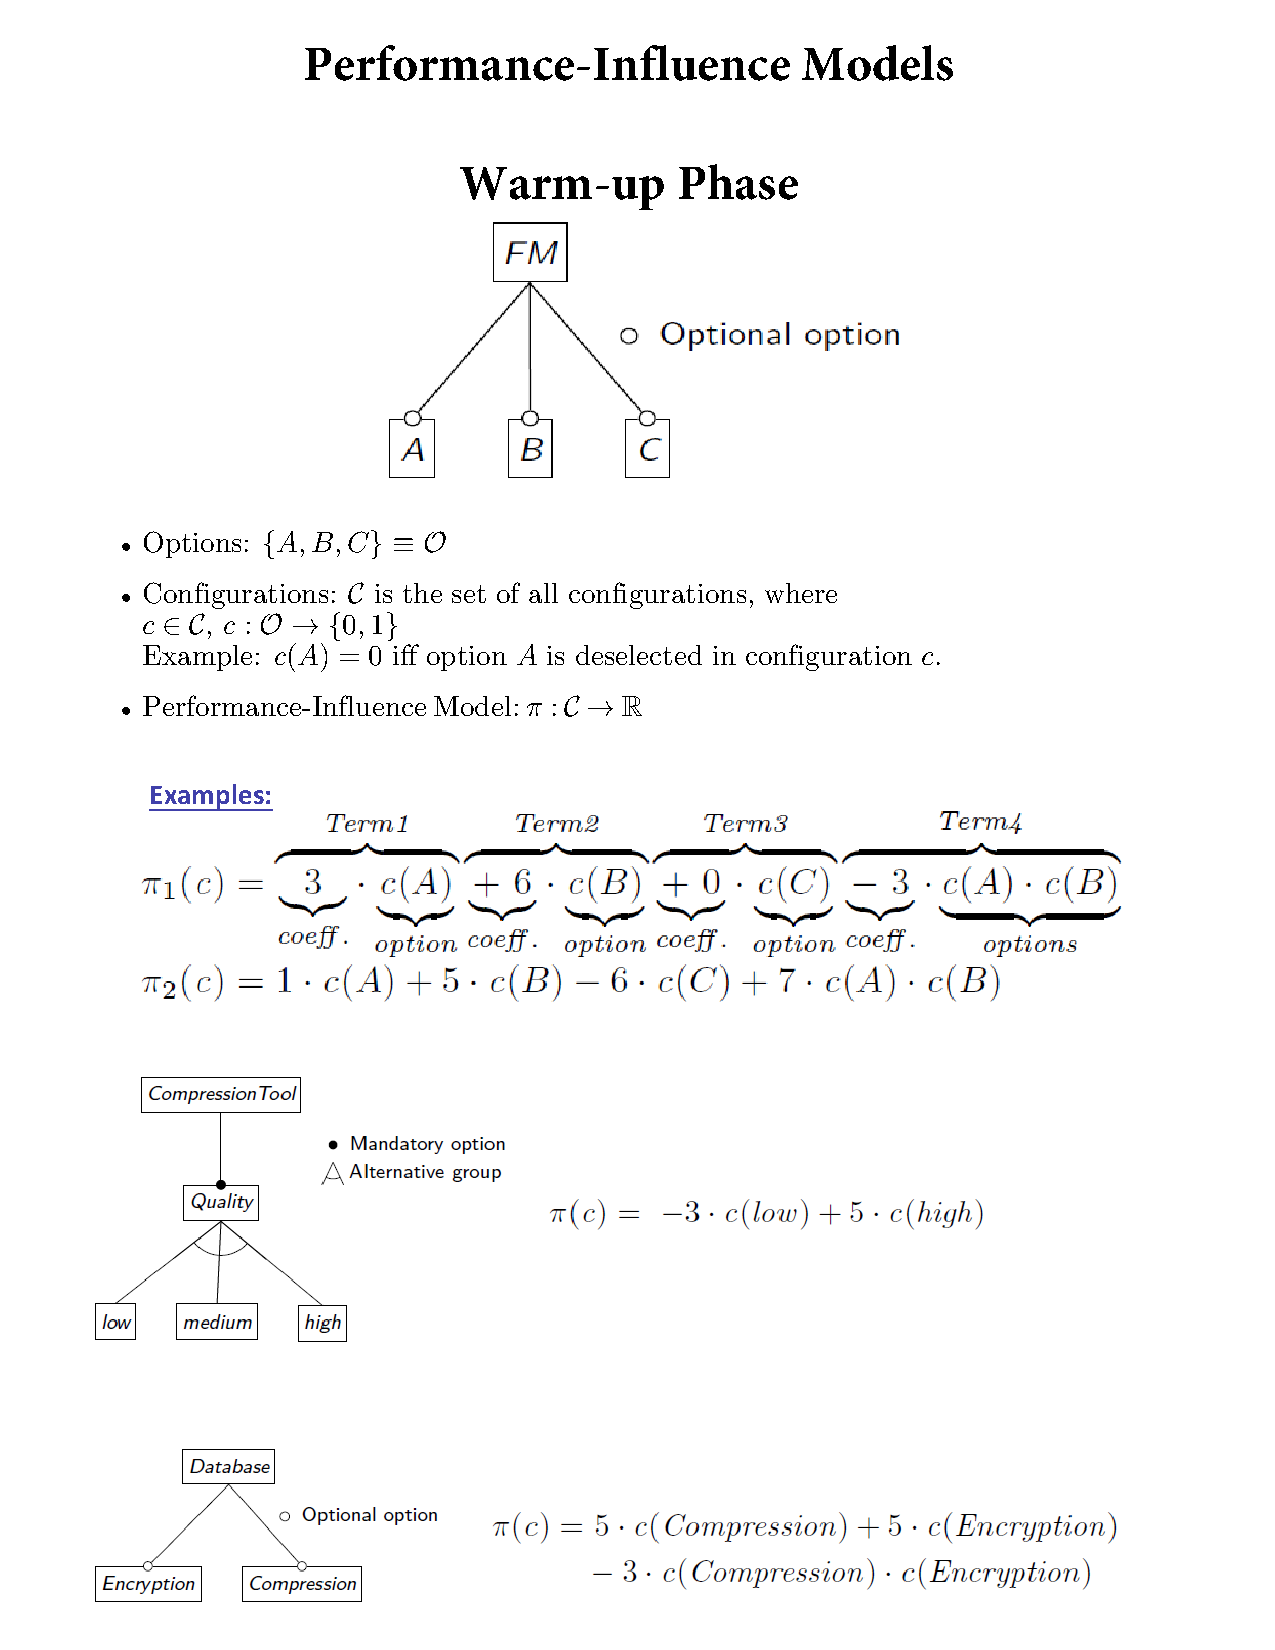
\includepdf[pages=-]{literature/Interview_Questionnaire.pdf}


%*********************************************************************%
% LITERATURE                                                          %
%*********************************************************************%

\cleardoublepage
\phantomsection 
\addcontentsline{toc}{chapter}{\bibname} % 
\bibliographystyle{alpha} % plain gerplain abbrvnat unsrtnat alphag alpha
% in a thesis you have space... use full names
\bibliography{literature/IEEEfull,literature/MYfull,literature/literature}
% in a paper, space is limited. use abreviations
%\bibliography{../literature/IEEEabrv,../literature/MYabrv,../literature/literature}

%*********************************************************************%
% ERKLÄRUNG                                                           %
%*********************************************************************%

\ifnotdraft{
	\cleardoublepage
	\phantomsection
	\printindex
	\thispagestyle{empty}
\vspace*{25\baselineskip}
\hbox to \textwidth{\hrulefill}
\par
\textbf{Eidesstattliche Erklärung:}

Hiermit versichere ich an Eides statt, dass ich diese Masterarbeit selbständig und
ohne Benutzung anderer als der angegebenen Quellen und Hilfsmittel angefertigt
habe und dass alle Ausführung\-en, die wörtlich oder sinngemäß übernommen wurden,
als solche gekenn\-zeichnet sind, sowie dass ich die Masterarbeit in gleicher oder
ähnlicher Form noch keiner anderen Prüfungsbehörde vorgelegt habe.

I hereby certify that this master’s thesis has been composed by myself, and describes my own work, unless otherwise acknowledged in the text. All references and verbatim extracts have been quoted, and all sources of information have been specifically acknowledged. It has not been submitted in any other application for a
degree.

\vspace*{20pt}

Rima Celita Lewis

Passau, den \thefullgermandate
%
% Hiermit erkl\"are ich, dass ich die vorliegende Arbeit selbst\"andig verfasst und
% keine anderen als die angegebenen Quellen und Hilfsmittel verwendet habe.
%
% Magdeburg, den \todots

%%%%%%%%%%%%%%%%%%%%%%%%%%%%%%%%%%%%%%%%%%%%%%%%%%%%%%%%%%%%%%%%%%%%%%%%
%% Hinweis:
%%
%% Diese Erklärung wird von der Prüfungsordnung für Diplomarbeiten
%% verlangt und ist zu unterschreiben. Für Studienarbeiten ist diese
%% Erklärung nicht zwingend notwendig, schadet aber auch nicht.
%%%%%%%%%%%%%%%%%%%%%%%%%%%%%%%%%%%%%%%%%%%%%%%%%%%%%%%%%%%%%%%%%%%%%%%%
\clearpage

}

\end{document}
